%# -*- coding: utf-8-unix -*-
%%==================================================
%% thesis.tex
%%==================================================

% 双面打印
\documentclass[master, openright, twoside]{sjtuthesis}
% \documentclass[bachelor, fontset=adobe, openany, oneside, submit]{sjtuthesis}
% \documentclass[master, fontset=adobe, review]{sjtuthesis}
% \documentclass[%
%   bachelor|master|doctor,	% 必选项
%   fontset=adobe|windows,  	% 只测试了adobe
%   oneside|twoside,		% 单面打印,双面打印(奇偶页交换页边距,默认)
%   openany|openright, 		% 可以在奇数或者偶数页开新章|只在奇数页开新章(默认)
%   zihao=-4|5,, 		% 正文字号:小四、五号(默认)
%   review,	 		% 盲审论文,隐去作者姓名、学号、导师姓名、致谢、发表论文和参与的项目
%   submit			% 定稿提交的论文,插入签名扫描版的原创性声明、授权声明 
% ]

\usepackage{thesisfonts_external}

% 逐个导入参考文献数据库
\addbibresource{bib/thesis.bib}
% \addbibresource{bib/chap2.bib}

\begin{document}

%% 无编号内容:中英文论文封面、授权页
%# -*- coding: utf-8-unix -*-
\title{基于信息熵的数据交易定价研究}
\author{李希君}
\advisor{姚建国副教授}
% \coadvisor{某某教授}
\defenddate{2014年12月17日}
\school{上海交通大学}
\institute{电子信息与电气工程学院}
\studentnumber{115037910069}
\major{软件工程}

\englishtitle{Information Entropy-based Data Pricing}
\englishauthor{\textsc{Xijun Li}}
\englishadvisor{Prof. \textsc{Jianguo Yao}}
% \englishcoadvisor{Prof. \textsc{Uom Uom}}
\englishschool{Shanghai Jiao Tong University}
\englishinstitute{\textsc{School of Electronic Information and Electrical Engineering} \\
  \textsc{Shanghai Jiao Tong University} \\
  \textsc{Shanghai, P.R.China}}
\englishmajor{Software Engineering}
\englishdate{Dec. 17th, 2014}


\maketitle

\makeenglishtitle

\makeatletter
\ifsjtu@submit\relax
	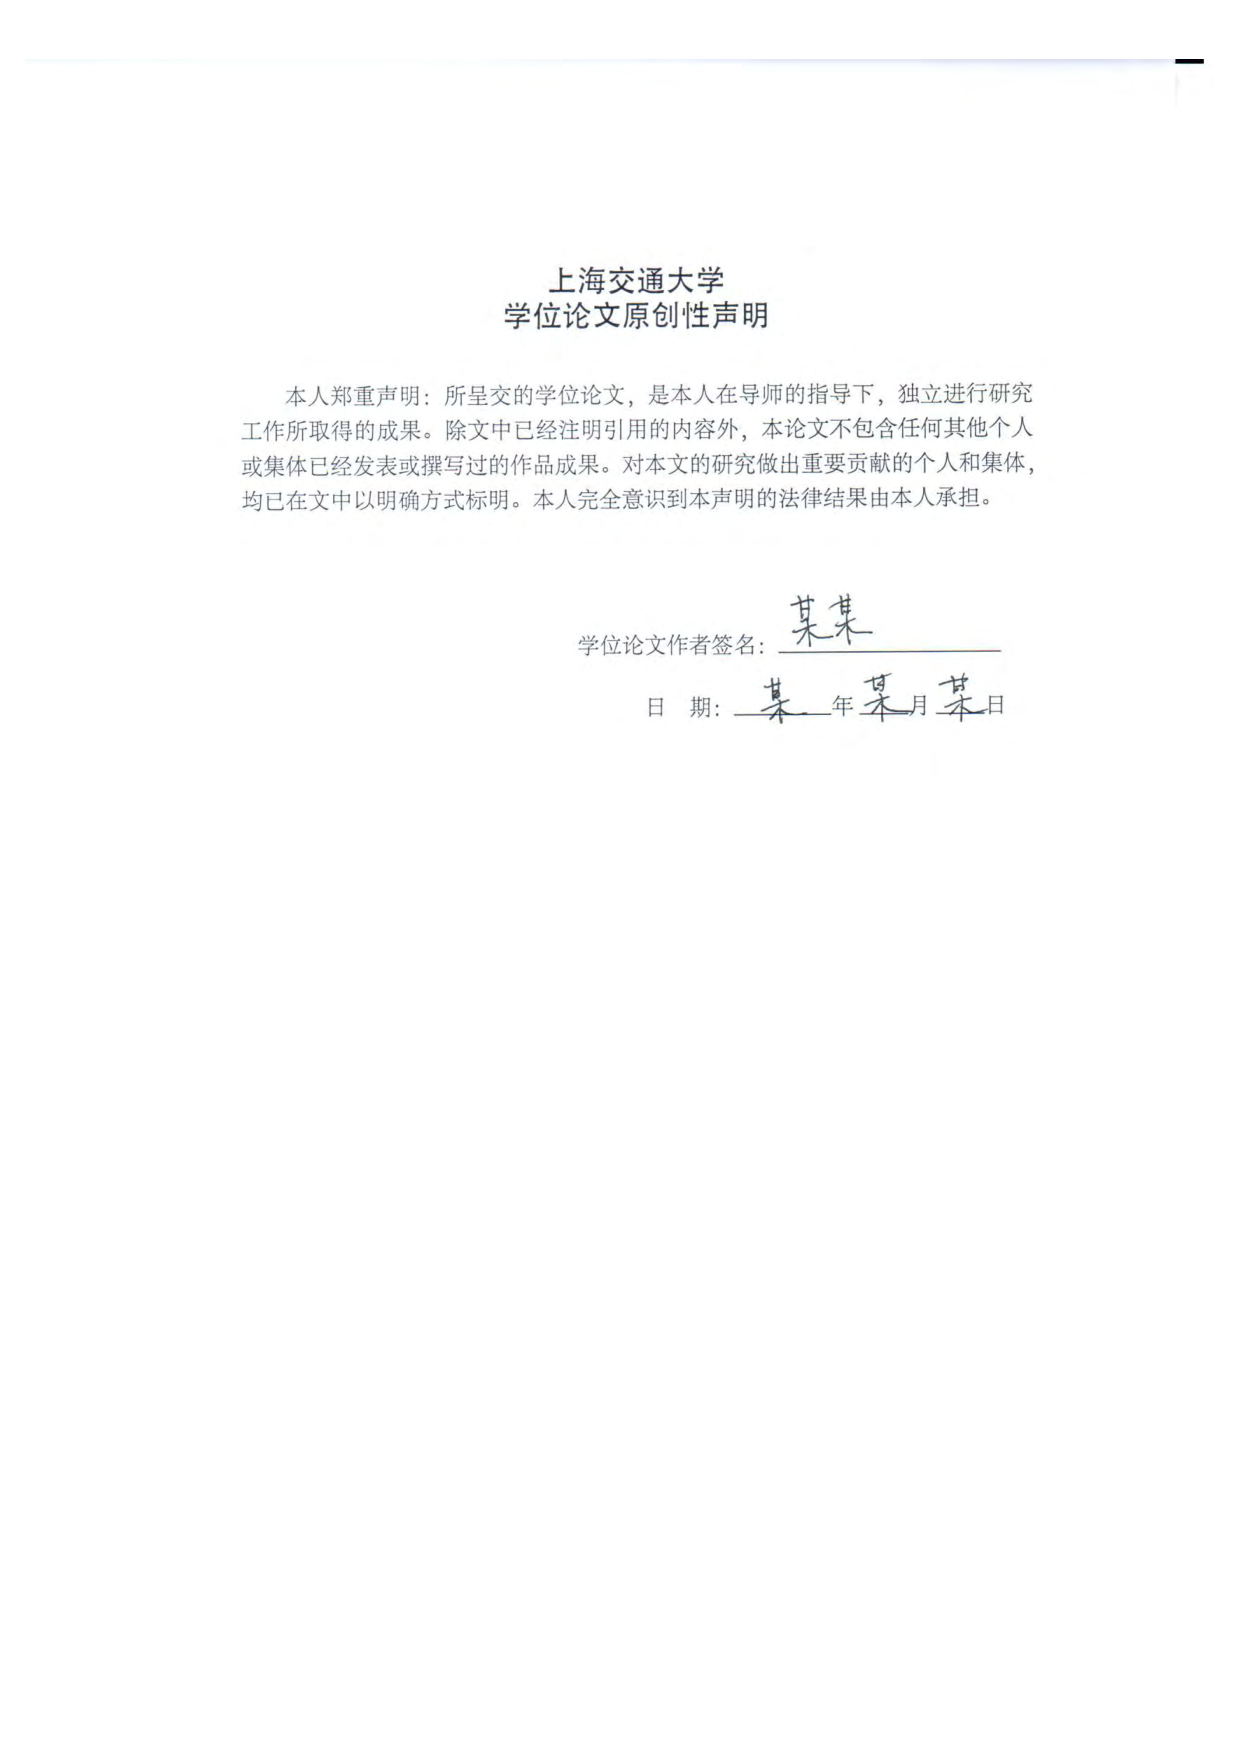
\includepdf{pdf/original.pdf}
	\cleardoublepage
	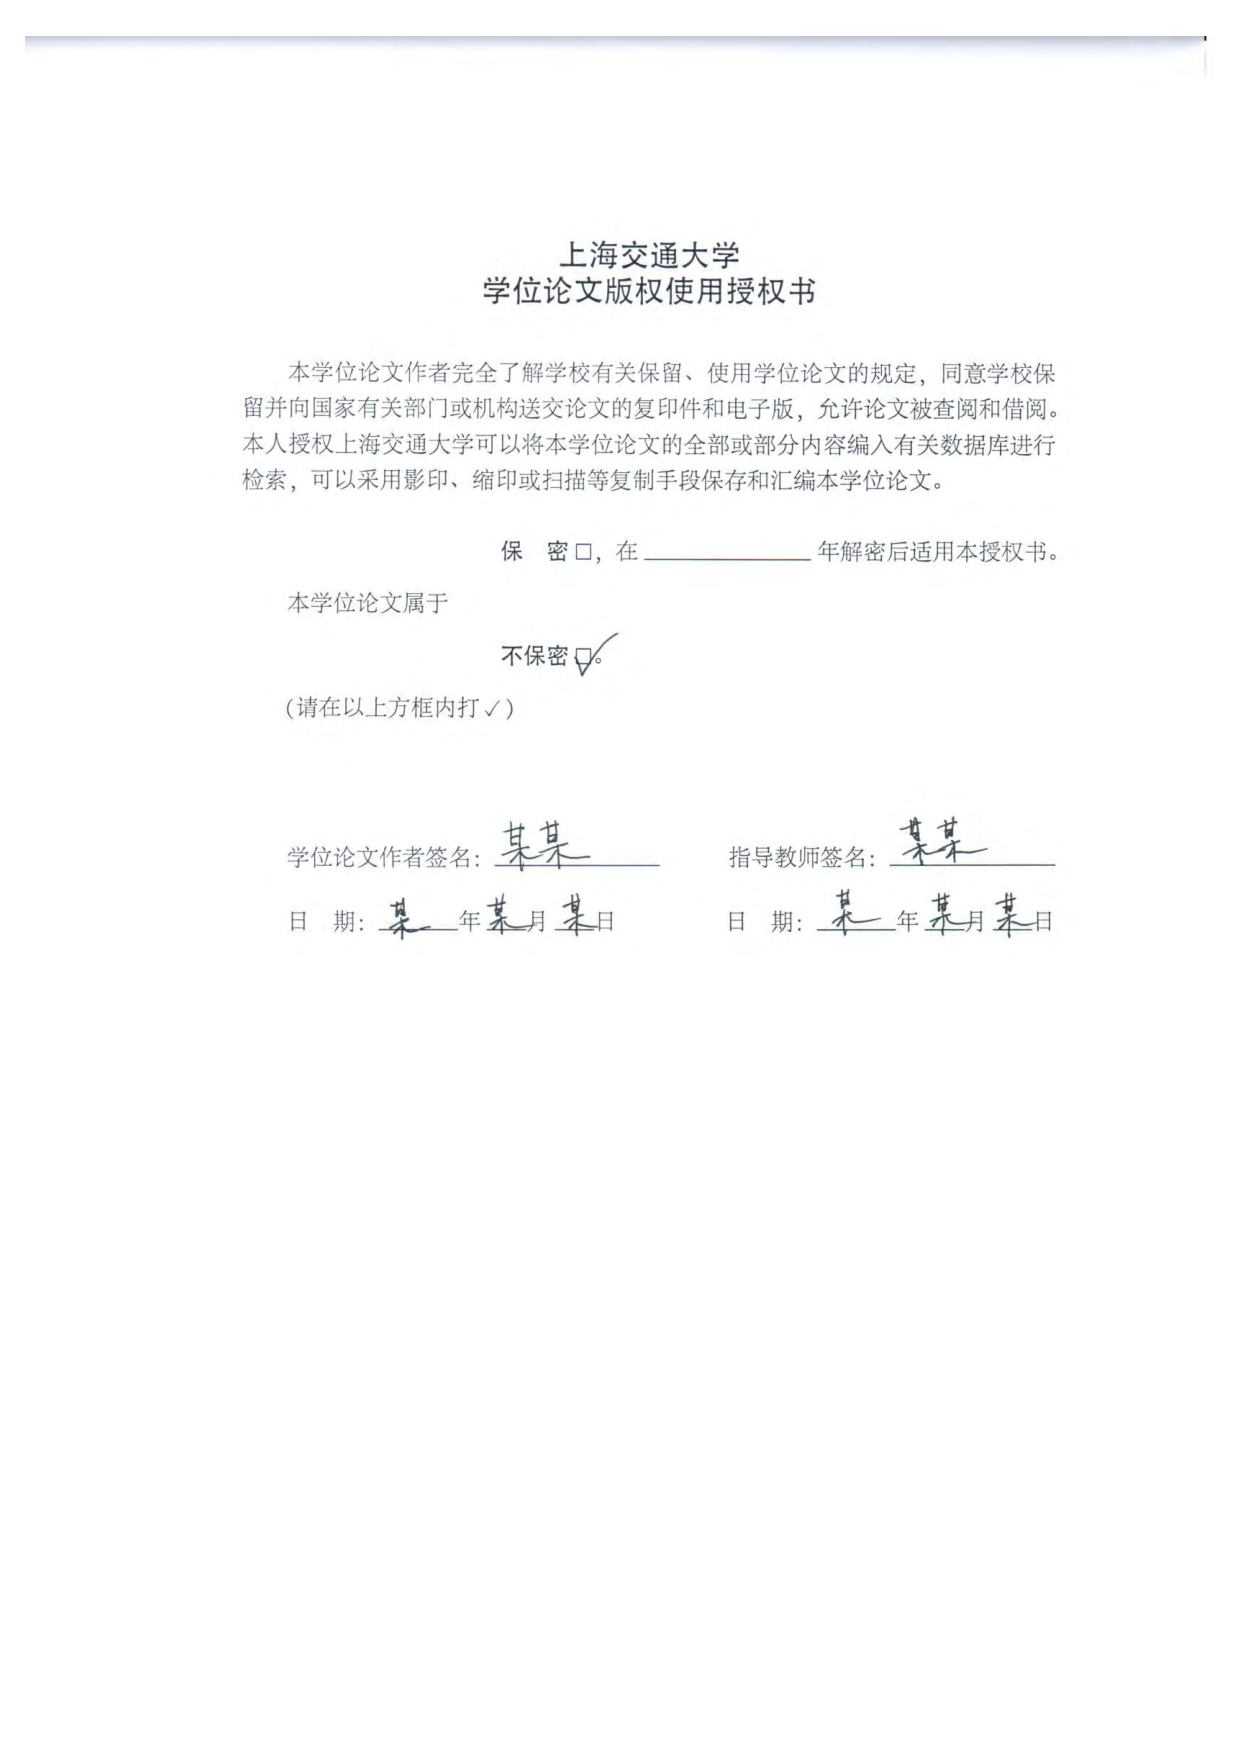
\includepdf{pdf/authorization.pdf}
	\cleardoublepage
\else
\ifsjtu@review\relax
% exclude the original claim and authorization
\else
	\makeDeclareOriginal
	\makeDeclareAuthorization
\fi
\fi
\makeatother


\frontmatter 	% 使用罗马数字对前言编号

%% 摘要
\pagestyle{main}
%# -*- coding: utf-8-unix -*-
%%==================================================
%% abstract.tex for SJTU Master Thesis
%%==================================================

\begin{abstract}

上海交通大学是我国历史最悠久的高等学府之一,是教育部直属、教育部与上海市共建的全国重点大学,是国家 “七五”、“八五”重点建设和“211工程”、“985工程”的首批建设高校。经过115年的不懈努力,上海交通大学已经成为一所“综合性、研究型、国际化”的国内一流、国际知名大学,并正在向世界一流大学稳步迈进。 

十九世纪末,甲午战败,民族危难。中国近代著名实业家、教育家盛宣怀和一批有识之士秉持“自强首在储才,储才必先兴学”的信念,于1896年在上海创办了交通大学的前身——南洋公学。建校伊始,学校即坚持“求实学,务实业”的宗旨,以培养“第一等人才”为教育目标,精勤进取,笃行不倦,在二十世纪二三十年代已成为国内著名的高等学府,被誉为“东方MIT”。抗战时期,广大师生历尽艰难,移转租界,内迁重庆,坚持办学,不少学生投笔从戎,浴血沙场。解放前夕,广大师生积极投身民主革命,学校被誉为“民主堡垒”。

新中国成立初期,为配合国家经济建设的需要,学校调整出相当一部分优势专业、师资设备,支持国内兄弟院校的发展。五十年代中期,学校又响应国家建设大西北的号召,根据国务院决定,部分迁往西安,分为交通大学上海部分和西安部分。1959年3月两部分同时被列为全国重点大学,7月经国务院批准分别独立建制,交通大学上海部分启用“上海交通大学”校名。历经西迁、两地办学、独立办学等变迁,为构建新中国的高等教育体系,促进社会主义建设做出了重要贡献。六七十年代,学校先后归属国防科工委和六机部领导,积极投身国防人才培养和国防科研,为“两弹一星”和国防现代化做出了巨大贡献。

改革开放以来,学校以“敢为天下先”的精神,大胆推进改革:率先组成教授代表团访问美国,率先实行校内管理体制改革,率先接受海外友人巨资捐赠等,有力地推动了学校的教学科研改革。1984年,邓小平同志亲切接见了学校领导和师生代表,对学校的各项改革给予了充分肯定。在国家和上海市的大力支持下,学校以“上水平、创一流”为目标,以学科建设为龙头,先后恢复和兴建了理科、管理学科、生命学科、法学和人文学科等。1999年,上海农学院并入;2005年,与上海第二医科大学强强合并。至此,学校完成了综合性大学的学科布局。近年来,通过国家“985工程”和“211工程”的建设,学校高层次人才日渐汇聚,科研实力快速提升,实现了向研究型大学的转变。与此同时,学校通过与美国密西根大学等世界一流大学的合作办学,实施国际化战略取得重要突破。1985年开始闵行校区建设,历经20多年,已基本建设成设施完善,环境优美的现代化大学校园,并已完成了办学重心向闵行校区的转移。学校现有徐汇、闵行、法华、七宝和重庆南路(卢湾)5个校区,总占地面积4840亩。通过一系列的改革和建设,学校的各项办学指标大幅度上升,实现了跨越式发展,整体实力显著增强,为建设世界一流大学奠定了坚实的基础。

交通大学始终把人才培养作为办学的根本任务。一百多年来,学校为国家和社会培养了20余万各类优秀人才,包括一批杰出的政治家、科学家、社会活动家、实业家、工程技术专家和医学专家,如江泽民、陆定一、丁关根、汪道涵、钱学森、吴文俊、徐光宪、张光斗、黄炎培、邵力子、李叔同、蔡锷、邹韬奋、陈敏章、王振义、陈竺等。在中国科学院、中国工程院院士中,有200余位交大校友;在国家23位“两弹一星”功臣中,有6位交大校友;在18位国家最高科学技术奖获得者中,有3位来自交大。交大创造了中国近现代发展史上的诸多“第一”:中国最早的内燃机、最早的电机、最早的中文打字机等;新中国第一艘万吨轮、第一艘核潜艇、第一艘气垫船、第一艘水翼艇、自主设计的第一代战斗机、第一枚运载火箭、第一颗人造卫星、第一例心脏二尖瓣分离术、第一例成功移植同种原位肝手术、第一例成功抢救大面积烧伤病人手术等,都凝聚着交大师生和校友的心血智慧。改革开放以来,一批年轻的校友已在世界各地、各行各业崭露头角。

截至2011年12月31日,学校共有24个学院/直属系(另有继续教育学院、技术学院和国际教育学院),19个直属单位,12家附属医院,全日制本科生16802人、研究生24495人(其中博士研究生5059人);有专任教师2979名,其中教授835名;中国科学院院士15名,中国工程院院士20名,中组部“千人计划”49名,“长江学者”95名,国家杰出青年基金获得者80名,国家重点基础研究发展计划(973计划)首席科学家24名,国家重大科学研究计划首席科学家9名,国家基金委创新研究群体6个,教育部创新团队17个。

学校现有本科专业68个,涵盖经济学、法学、文学、理学、工学、农学、医学、管理学和艺术等九个学科门类;拥有国家级教学及人才培养基地7个,国家级校外实践教育基地5个,国家级实验教学示范中心5个,上海市实验教学示范中心4个;有国家级教学团队8个,上海市教学团队15个;有国家级教学名师7人,上海市教学名师35人;有国家级精品课程46门,上海市精品课程117门;有国家级双语示范课程7门;2001、2005和2009年,作为第一完成单位,共获得国家级教学成果37项、上海市教学成果157项。

\keywords{\large 上海交大 \quad 饮水思源 \quad 爱国荣校}
\end{abstract}

\begin{englishabstract}

An imperial edict issued in 1896 by Emperor Guangxu, established Nanyang Public School in Shanghai. The normal school, school of foreign studies, middle school and a high school were established. Sheng Xuanhuai, the person responsible for proposing the idea to the emperor, became the first president and is regarded as the founder of the university.

During the 1930s, the university gained a reputation of nurturing top engineers. After the foundation of People's Republic, some faculties were transferred to other universities. A significant amount of its faculty were sent in 1956, by the national government, to Xi'an to help build up Xi'an Jiao Tong University in western China. Afterwards, the school was officially renamed Shanghai Jiao Tong University.

Since the reform and opening up policy in China, SJTU has taken the lead in management reform of institutions for higher education, regaining its vigor and vitality with an unprecedented momentum of growth. SJTU includes five beautiful campuses, Xuhui, Minhang, Luwan Qibao, and Fahua, taking up an area of about 3,225,833 m2. A number of disciplines have been advancing towards the top echelon internationally, and a batch of burgeoning branches of learning have taken an important position domestically.

Today SJTU has 31 schools (departments), 63 undergraduate programs, 250 masters-degree programs, 203 Ph.D. programs, 28 post-doctorate programs, and 11 state key laboratories and national engineering research centers.

SJTU boasts a large number of famous scientists and professors, including 35 academics of the Academy of Sciences and Academy of Engineering, 95 accredited professors and chair professors of the "Cheung Kong Scholars Program" and more than 2,000 professors and associate professors.

Its total enrollment of students amounts to 35,929, of which 1,564 are international students. There are 16,802 undergraduates, and 17,563 masters and Ph.D. candidates. After more than a century of operation, Jiao Tong University has inherited the old tradition of "high starting points, solid foundation, strict requirements and extensive practice." Students from SJTU have won top prizes in various competitions, including ACM International Collegiate Programming Contest, International Mathematical Contest in Modeling and Electronics Design Contests. Famous alumni include Jiang Zemin, Lu Dingyi, Ding Guangen, Wang Daohan, Qian Xuesen, Wu Wenjun, Zou Taofen, Mao Yisheng, Cai Er, Huang Yanpei, Shao Lizi, Wang An and many more. More than 200 of the academics of the Chinese Academy of Sciences and Chinese Academy of Engineering are alumni of Jiao Tong University.

\englishkeywords{\large SJTU, master thesis, XeTeX/LaTeX template}
\end{englishabstract}



%% 目录、插图目录、表格目录
\tableofcontents
\listoffigures
\addcontentsline{toc}{chapter}{\listfigurename} %将插图目录加入全文目录
\listoftables
\addcontentsline{toc}{chapter}{\listtablename}  %将表格目录加入全文目录
\listofalgorithms
\addcontentsline{toc}{chapter}{算法索引}        %将算法目录加入全文目录

%# -*- coding: utf-8-unix -*-
\chapter{主要符号对照表}
\label{chap:symb}

\begin{longtable}{rl}
$\epsilon$     & 介电常数 \\
 $\mu$ 		& 磁导率 \\
 $\epsilon$     & 介电常数 \\
 $\mu$ 		& 磁导率 \\
 $\epsilon$     & 介电常数 \\
 $\mu$ 		& 磁导率 \\
 $\epsilon$ 	& 介电常数 \\
 $\mu$ 		& 磁导率 \\
 $\epsilon$     & 介电常数 \\
 $\mu$ 		& 磁导率 \\
 $\epsilon$     & 介电常数 \\
 $\mu$ 		& 磁导率 \\
 $\epsilon$     & 介电常数 \\
 $\mu$ 		& 磁导率 \\
 $\epsilon$ 	& 介电常数 \\
 $\mu$ 		& 磁导率 \\
 $\epsilon$     & 介电常数 \\
 $\mu$ 		& 磁导率 \\
 $\epsilon$     & 介电常数 \\
 $\mu$ 		& 磁导率 \\
 $\epsilon$     & 介电常数 \\
 $\mu$ 		& 磁导率 \\
 $\epsilon$ 	& 介电常数 \\
 $\mu$ 		& 磁导率 \\
 $\epsilon$     & 介电常数 \\
 $\mu$ 		& 磁导率 \\
 $\epsilon$     & 介电常数 \\
 $\mu$ 		& 磁导率 \\
 $\epsilon$     & 介电常数 \\
 $\mu$ 		& 磁导率 \\
 $\epsilon$ 	& 介电常数 \\
 $\mu$ 		& 磁导率 \\
 $\epsilon$     & 介电常数 \\
 $\mu$ 		& 磁导率 \\
 $\epsilon$     & 介电常数 \\
 $\mu$ 		& 磁导率 \\
 $\epsilon$     & 介电常数 \\
 $\mu$ 		& 磁导率 \\
 $\epsilon$ 	& 介电常数 \\
 $\mu$ 		& 磁导率 \\
 $\epsilon$     & 介电常数 \\
 $\mu$ 		& 磁导率 \\
 $\epsilon$     & 介电常数 \\
 $\mu$ 		& 磁导率 \\
 $\epsilon$     & 介电常数 \\
 $\mu$ 		& 磁导率 \\
 $\epsilon$ 	& 介电常数 \\
 $\mu$ 		& 磁导率 \\
 $\epsilon$     & 介电常数 \\
 $\mu$ 		& 磁导率 \\
 $\epsilon$     & 介电常数 \\
 $\mu$ 		& 磁导率 \\
 $\epsilon$     & 介电常数 \\
 $\mu$ 		& 磁导率 \\
\end{longtable}
 % 主要符号、缩略词对照表

\mainmatter	% 使用阿拉伯数字对正文编号

%% 正文内容
\pagestyle{main}
\chapter{研究背景}

近些年来,数据量的巨幅增长,尤其是从2005年到2010年,全球产生的数据量增长了10倍(从130艾字节增长到了1227艾字节),目前仍在继续增长\cite{gantz2012digital,villars2011big}。数据交易的市场也以惊人的速度发展着,预计从目前到2020年,大数据和其商业分析的市场规模会从1301亿美元增长到2030亿美元\cite{idc}。如今,高质量和可信赖的数据商品及其相关的分析业务有着巨量的市场需求\cite{gantz2012digital,maitland2002european,turner2014digital,villars2011big}。

\begin{figure}[!htp]
  \centering
  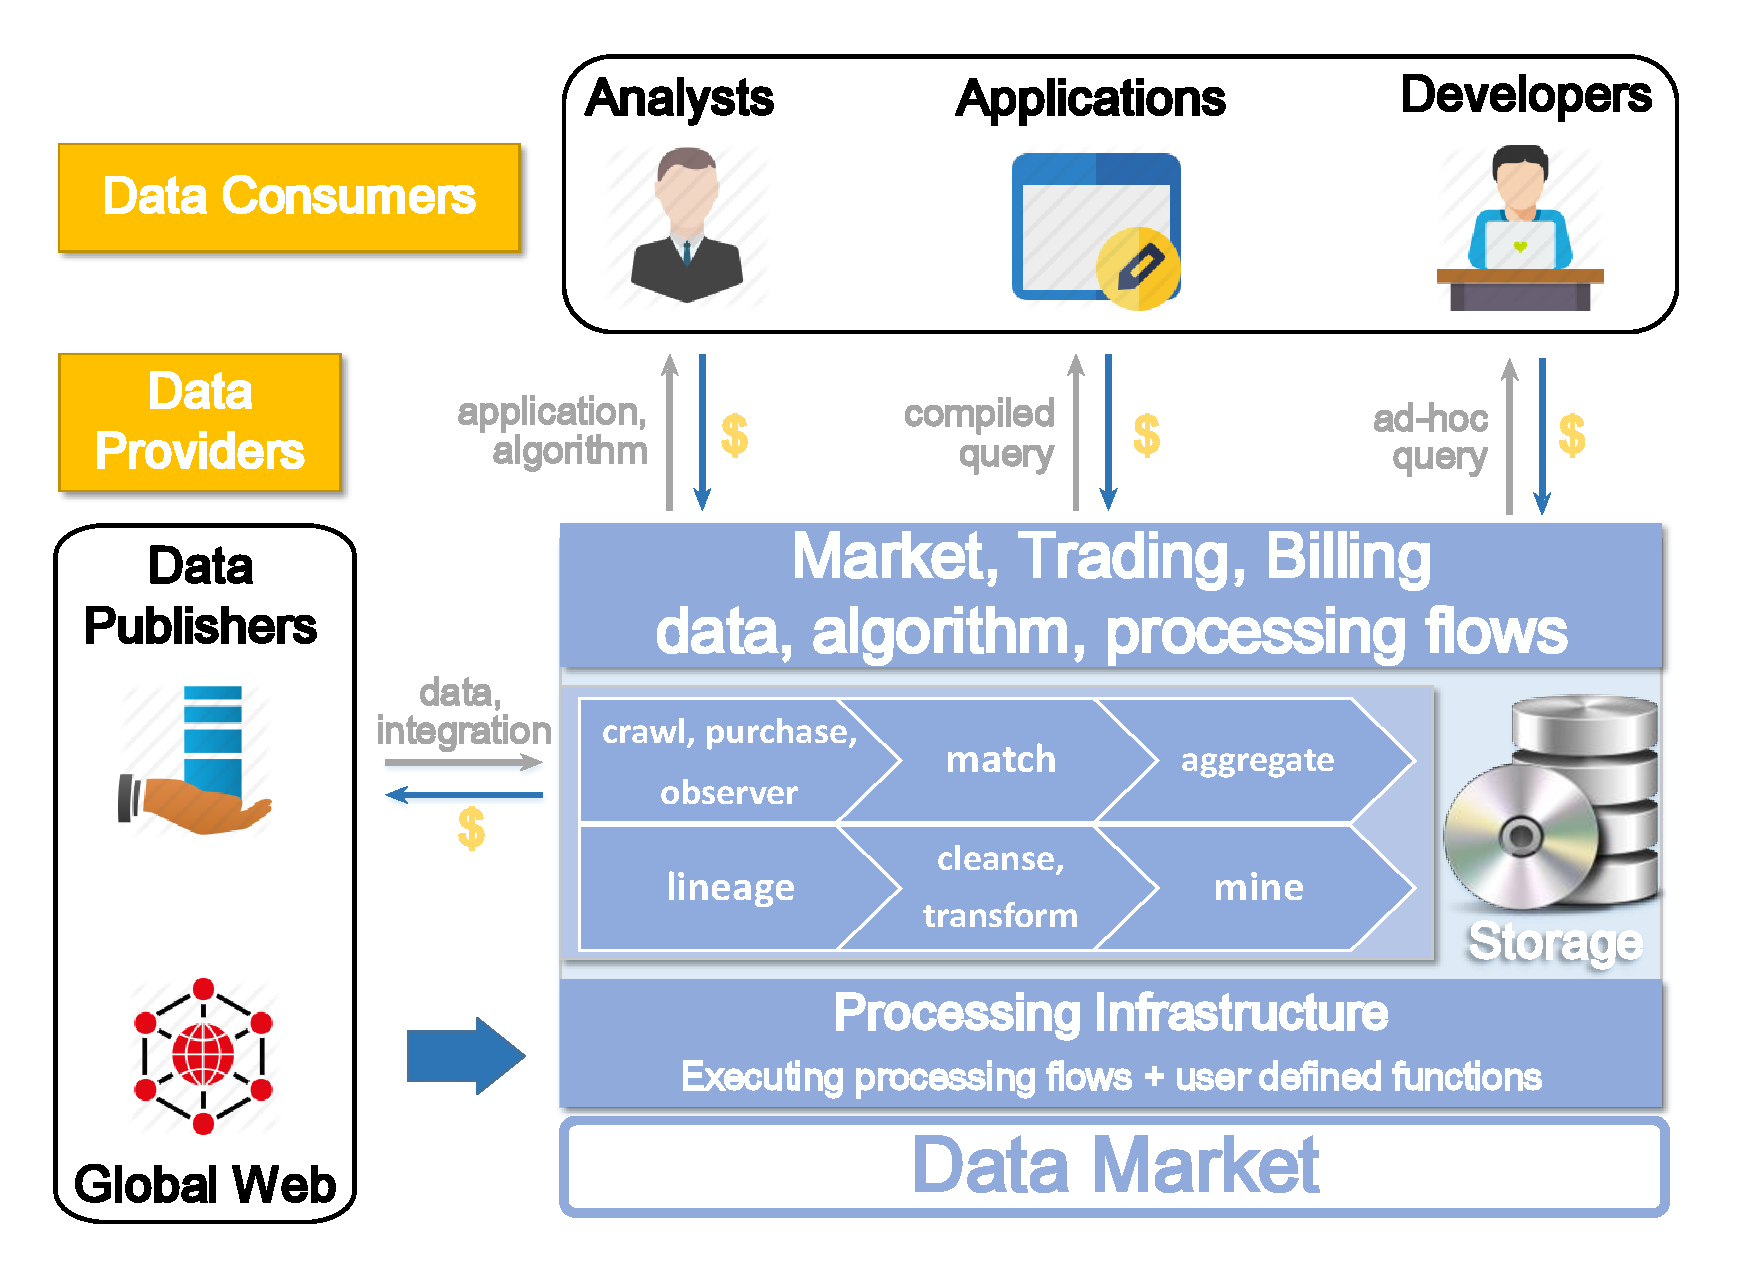
\includegraphics[width=0.65\textwidth]{chapter1/data_market_flow.pdf}
  \bicaption[fig:data market flow]{数据市场数据流动示意图}{数据市场数据流动示意图}{Fig}{Data Flow in Data Market}
\end{figure}

现在,数据商品和相关分析业务主要是由在线数据市场提供的。这些市场从数据发布者和全球网络收集数据,并对其进行清洗、挖掘和整理,然后出售给不同的消费者,如图\ref{fig:data market flow}所示。具体来说,数据消费者主要由开发者和中小企业主构成。这些数据消费者需要在线数据市场提供的数据和相关分析业务来帮助他们做商业决策。至于在线数据市场,他们在整理过的、有价值的数据的基础上,提供分析、商业应用和算法等服务给消费者。现在,国外主要有三家数据交易平台,分别是Microsoft Windows Azure Data Marketplace\cite{MicrosoftAzure}, Inforchimps\cite{infochimps}以及Factual\cite{factual}。而国内也主要有三家平台,分别是贵阳大数据交易所\cite{gbdex},武汉长江大数据交易中心和武汉东湖大数据交易中心\cite{chinadatatrading}。然而,在这些国内外数据交易平台,并没有一个统一的定价机制来指导整个市场。因此,当前数据产品的定价处于一个比较混乱的阶段。不同的数据交易平台采用的是不同的定价机制,而其中最普遍采用的有四种种机制:基于订阅的定价机制、基于查询的定价机制,捆绑销售定价机制以及私下协商定价机制。选择什么样的定价机制具体取决于消费者使用模式以及数据提供商之间的竞争差异。但是,需要指出的是,目前没有任何一种定价机制将数据本身所含有的信息量考虑为定价因素。从消费者角度考虑,目前很多数据消费者通常只对市场上数据集的某些子集感兴趣,他们并不需要购买完整的数据集,而交易平台往往给出的是完整数据集的价格。当消费者购买这些子集时,他们需要知道这些子集所含信息占完整数据集的比例从而评估交易平台给出的子集定价是否合理。从数据交易平台的角度看,如果他们能给出更多的子集数据价格以及它们之间的信息量关系的话,就能给消费者提供一个更加透明的定价关系,从而吸引更多的消费者进行消费。另一方面,目前已有的定价机制并不能产生最大交易剩余,这样会降低买卖双方的交易信心,从而使原本能发生的交易而没有发生,这将会对数据及其相关交易带来极大的经济损失。因此,我们进行了基于信息熵的数据交易的研究课题,期望以数据产品本身的信息量作为定价指标,然后基于这一指标探索更合适的交易机制,从而更好地促进数据交易市场的发展。

\chapter{国内外研究现状}

\section{国外主流在线数据交易平台}

Microsoft Windows Azure Data Marketplace\cite{MicrosoftAzure}在2010年正式成立,微软将其作为Azure云平台的一部分。Azure Data Marketplace非常善于将数据买家与数据发布者联系在一起。因此,几个主要的国外数据提供商比如ESRI, Dun and Bradstreet 都能在这个平台被找到。在Azure Data Marketplace上的所有数据集大致可以分为两类:免费和收费。这两种数据集都是需要消费者订阅才能有权限查阅或使用这些数据集的。对于免费的数据集,数据买家可以每月无限次数的访问它们,但在它们上定义的查询事务数量是有限的。而对于收费的数据集来说,数据买家需要根据每月访问次数来支付一定费用才能访问它们。通过使用一个标准的数据协议Odata,这个平台给数据买家提供了一个定义良好的网络接口来访问平台中的数据。然而,对于Azure Data Marketplace上的数据发布者,微软并没给出具体的定价建议,尤其是多个数据发布者存在竞争的局面时。

Infochimps\cite{infochimps}数据交易平台成立于2009年,它最初的目标是去收集尽可能多的公开的商业数据集。Factual\cite{factual}成立于2007年,它主要致力于在地理信息数据的收集和售卖。与Azure Data Marketplace存在同样的问题是,这二者都没有为平台上的数据发布商提供一个明确的定价策略建议。在Infochimps和Factual上,数据买家在购买自己想要的数据时只能去直接联系平台上的数据发布商,经协商后确定数据价格。这么看来,数据交易平台只是起到了一个中介的作用,最终的数据交易价格并不是统一和透明的。在表\ref{tab:comparison_datamarket}中,我们给出上述三个交易平台的详细比较。

\begin{table}[h]
\centering
\bicaption[tab:comparison_datamarket]{三个国外主要数据市场的比较}{三个国外主要数据市场的比较}{Table}{Comparison for three major data markets}
 \begin{tabular}{|p{2.5cm}|p{2.5cm}|p{2.5cm}|p{2.5cm}|}
        \hline
               & Azure~\cite{MicrosoftAzure} & Infochimps~\cite{infochimps} & Factual~\cite{factual} \\
        \hline
        \hline
          数据类型  & 多种类型 & 主要是地理数据 & 主要是地理、社交以及网络数据 \\
        \hline
          数据免费  & 是 & 是 & ---\\
        \hline
          付费数据的免费试用  & 是 & --- & 是,但仅供API免费试用 \\
        \hline
          交付方式  & OData API & API, 下载 & API, 为重度用户提供下载\\
        \hline
          应用部署  & Windows Azure & Infochimps自建平台 & --- \\
        \hline
          数据发布  & 通过网络服务或者连接数据库 & 上传 & 上传 \\
        \hline
        成立时间  & 2010 & 2009 & 2007 \\
        \hline
 \end{tabular}
\end{table}

\section{国内主流在线数据交易平台}

贵阳大数据交易所\cite{gbdex}成立于2014年12月31日,2015年4月14日正式挂牌运营,是我国乃至全球第一家大数据交易所。秉承“贡献中国数据智慧 释放全球数据价值”发展理念,志在成为全球最重要的交易所,旨在推动政府数据公开、行业数据价值发现。截至2016年9月1日,交易额累积突破1亿元,交易框架协议接近3亿元,发展会员超过500家,可交易数据产品接近4000个,可交易的数据总量超过60PB。贵阳大数据交易所交易的并不是底层数据,而是基于底层数据,通过数据的清洗、分析、建模、可视化出来的结果, 彻底解决了数据如何保护隐私及数据所有权的问题。 贵阳大数据交易所将成为永不休市的交易所, 将实行7×24小时的交易时间。其涉及的数据类型有金融、政府、医疗、社会、海关、能源、社交、商品、水电煤、法院、交通、企业、通信、银行卡、专利等。

武汉长江大数据交易中心是在武汉市委市政府支持下设立的、第三方中立的、具有公信力的大数据交易中心,是武汉市政府推出的“互联网+”产业创新工程“11711”行动计划中关于大数据产业发展的重要部署。武汉长江大数据交易中心采用市场化的运作方式,以推动政府及社会各领域数据的开放、融合为宗旨,以大数据应用为导向,汇聚数据清洗、数据加工、数据咨询、数据创意等全产业链资源,沉淀数据分析技术和供需场景,将多维度数据源与业务逻辑无缝衔接,逐步构建大数据交易生态,解决数据流通困局,让大数据真正成为推动区域经济转型升级的强大动力。

武汉东湖大数据交易中心\cite{chinadatatrading}成立于2015年7月,是经武汉市政府批准成立的华中地区首家大数据交易机构,也是国内最早探索并实施"政务数据运营解决方案"的服务机构,注册资金6000万元。东湖大数据联合武汉市互联网信息办公室和武汉市国有资产管理公司制订《武汉市政务数据资产运营中心成立方案》,参与筹建"武汉市政务数据资产运营中心",将成为全国首个以政务行业为主的大数据运营机构,将参与相关标准、规则的制定,来促进政府数据开放,带动整个产业链的发展。交易中心由具有政府背景的——武汉国有资产经营公司;领先的数据资产运营商——中润普达;优秀的地理空间信息公司——武大吉奥,及武汉市智慧产业投资公司、汉口银行等行业领军企业共同组建。交易中心目前整合的大数据覆盖了200多个行业、30大品类,实现了数千万条数据的汇集。截止2016年5月,已经服务了近百个省市区政府、金融机构、产业集团等客户。涉及到的数据集类型有交通环境、公共服务、健康医疗、金融商贸、科研应用、社交征信、科研应用、文娱音乐、知识产权、智慧生活、产业数据、政府数据。


\section{已有的数据定价策略}

基于订阅的定价机制是一个传统的数据商品定价机制。在那些实行订阅定价机制的数据交易平台,数据买家需要根据预先设定的事务数支付访问数据的费用。Azure Data Market就是一个很好的例子来解释这种定价机制。Azure有两种按月订阅类型:有限型和无限型。表\ref{tab:azure_tariff}给出了Azure Data Market的一个具体的价目表。比如数据集2010 Key US Demographics就是完全受限类型。如果一个数据买家想要每个月访问这个数据集10次,那么他就要支付$\$$9.95。然而,数据集EU Health Data Service UK和Business Verification就与2010 Key US Demographics稍有不同了,因为他们是部分受限类型的。数据买家可以每个月以免费的价格访问EU Health Data Service UK 5次或者Business Verification 10次。一旦数据买家访问这些数据集超过相应的免费访问次数,那么他也会被收取相应的费用。虽然,数据拥有者能比较容易地采用基于订阅制的定价机制来给商品定价,但是如果订阅价格设计的不够精密时,就会出现套利现象,从而给数据卖家带来经济损失,同时也会对其他没有套利的买家造成不公平。

\begin{table}[h]
\centering
\bicaption[tab:azure_tariff]{Azure数据市场部分商品价目表}{Azure数据市场部分商品价目表}{Table}{Datasets tariff in Azure data market}

    \begin{tabular}{|c|c|l|}
     \hline
               Dataset~\cite{MicrosoftAzure}& Transaction Limit& Price Level \\
     \hline
     \hline
        \multirow{3}{2cm}{2010 Key US Demographics}

                & $10$ &$\$9.95$\\
                & $50$ &$\$24.95$\\
                & $150$ &$\$49.95$\\
         \hline
         \multirow{3}{2cm}{EU Health Data Service UK}

                & $5$ &$\$0.00$\\
                & $100$ &$\$293.09$\\
                & $200$ &$\$732.83$\\
         \hline
         \multirow{4}{2cm}{Business Verification}
                & $100$ &$\$0.00$\\
                & $200$ &$\$100.00$\\
                & $2,500$ &$\$1,250.00$\\
                & $5,000$ &$\$2,425.00$\\
        \hline
 \end{tabular}
\end{table}


基于查询的定价机制是来源于关系数据库中的query。最近,一些数据交易平台开始采用这种机制来售卖他们的数据集。具体来说,数据买家为其想要的数据集向数据平台发起不同的特定的请求,而数据平台返回相应数据集的视图作为查询结果给数据买家,数据卖家根据查询的复杂度收取一定的费用。比如,CustomList\cite{customlists}以$\$$399售卖其全美商业数据库。数据买家可能只在意该数据集中有邮件地址的公司的数据子集,那么买家就向交易平台发起这么一个查询,交易平台查到相应视图返回结果并向买家收取$\$$299。然而,现在的数据交易平台并不支持复杂的查询操作,因为目前仍然并不清楚如何给不同的查询结果定一个合适的价格。Koutris\cite{koutris2015query}等人提出了一个基于查询的数据定价框架,该框架允许卖家给一些基本视图事先赋一些价格,然后当买家发起查询时,将查询到的基本视图的价格的和作为查询费用。但是,他们的工作仍旧没有解决如何给数据集的基本视图赋予合适价格的问题。

捆绑销售定价机制是起源于资本数据市场,它代表了一种聚合技术\cite{bakos2001aggregation}。在资本数据市场中,卖家经常将其多种产品捆绑,并对不同的客户以不同的价格销售。因此,这就会产生价格歧视效应\cite{bakos1999bundling}。举例来说,Dow Jones是一个金融信息公司,它将其信息和其他在线服务(比如新闻邮件推送服务,对特定公司的新闻实行监控和过滤服务)。Dow Jones为订阅者免费提供部分信息服务,但如果订阅者想要检索信息的全部内容,就需要开始付费了。此外,现在一些信息公司也开始实施了根据信息内容深度进行区别定价的策略。比如,Dow Jones对新闻的标题收费$\$$0.20,对新闻摘要收费$\$$1.00,对完整的新闻收费$\$$3.50。需要指出的是只有当捆绑的产品具有负相关性时,捆绑销售策略才能被市场接受。对于文本信息商品,比如新闻、文章,人们能比较弄清地分辨标题、摘要和全文的关系,然后根据内容深度的不同来给它们定价。但是,现如今,大部分的信息商品是非结构化的数据,比如音频、图像和视频。数据拥有者想要辨清这些数值数据的内在关系是困难的,因此想要根据信息深度来定价是不太可行的。

 \section{商品在线拍卖}

拍卖一个古老但有效的定价机制,它最早出现在公元前500年。大量的商品通过拍卖这一形式被交易。William Vickrey是第一个提出系统的拍卖理论的研究者\cite{Vickrey1961Counterspeculation}。之后,在Vickrey的理论基础上,涌现了更多拍卖的研究工作\cite{Milgrom1989Auctions,Milgrom1982A,Riley1981Optimal}。Riley等人\cite{Riley1981Optimal}在拍卖者独立同分布假设下研究了最优拍卖的性质。具体来说,他们比较了不同拍卖机制下卖家的期望收益。他们发现对于多数拍卖规则,如果卖家不接受低于保留价的报价时,英式拍卖或者荷兰式拍卖能最大化卖家期望收益。

互联网的快速发展使得传统商品的在线拍卖变成了可能,最早的在线拍卖出现在1993年\cite{Lucking2000Auctions}。目前出现了一大批在线拍卖市场,比如国外的eBay Live Auction\footnote{eBay Live Auction官方网站: \url{https://www.ebay.com/rpp/live-auctions}},国内的淘宝拍卖会\footnote{淘宝拍卖会官方网站: \url{https://paimai.taobao.com}}。大多数关于在线拍卖的理论研究都集中于B2C (Business-to-Customer) 或者C2C (Customer-to-Customer)的。这很大原因是研究者本身充当的角色多数是Customer。Beam等人\cite{Beam1998Auctions}使用搜索引擎分析了100个B2C和C2C在线拍卖实例,Riley等人\cite{Riley1981Optimal}也通过类似的方式分析了142个B2C和C2C拍卖实例。他们两组人的研究得到了一些相似的结论,即目前在线数据拍卖只使用了传统且有限的四组拍卖机制:英式拍卖,荷兰式拍卖,第一价格拍卖,以及Vickrey拍卖。在文献\cite{Lucking2000Auctions}中,Lucking认为传统拍卖理论的假设是不适用于新兴出现的在线拍卖的。在线拍卖是非常不同于传统拍卖的。一些因素,比如拍卖持续时长、竞拍人数、拍卖起价和保留价等在传统拍卖和在线拍卖中起的作用不尽相同。Pinker等人\cite{Pinker2003Managing,Pinker2001Using}称延长在线拍卖时长能有助于抬高成交价。Roth等人\cite{Roth2002Last}研究发现延迟进入拍卖 (late bidding) 和狙击拍卖 (snipe bidding) 在在线拍卖场景中时常发生。Reiley等人\cite{Ockenfels2006Online}发现设置公开的起拍价和保留价会减少竞拍人数且会使得竞拍物品流拍的可能性增大。此外,Ariely\cite{Dan2003Buying}也发现起拍价和最终成交价有着正相关关系。

大多数传统商品都是通过标的价格进行售卖的,但越来越多的物品开始通过拍卖这种机制来进行交易。在实践中,交易参与者们越来越多地认识到这种交易机制的好处。尽管大多数消费者对标的价格交易机制很熟悉而且也默认这种机制为大多数物品的交易方式,但是从交易量上来说,这是一个错误的认知。如果物品的交易成本和复杂度越高,则该物品越有可能通过拍卖的方式进行交易\cite{Pinker2003Managing}。此外,拍卖成交价能真实反映拍卖胜者的支付意愿,这能最大化拍卖参与者的总剩余。Lu等人\cite{Lu1996The}总结了这些通过拍卖交易的商品的共同特性:1、唯一性;2、不确定均衡价格。数据商品恰好符合这两个特性。在目前的在线数据市场,买家的数量远远大于卖家数量,这意味着数据交易市场是一个不完全竞争市场,近似于寡头市场。Harris等人\cite{Harris1981A}发现当市场需求超过供应时,拍卖也许是最好的交易机制。大量事实表明拍卖也许是一个对数据商品定价能起到最佳指导的机制。近些年来,大量关于传统商品的在线拍卖的研究\cite{Pinker2003Managing,Lucking2000Auctions,Pinker2001Using,Ockenfels2006Online,Dan2003Buying},例如邮票、古董等。然后传统商品的在线拍卖的经验是不能直接移植到数据商品上。另一方面,因为缺乏足够多的对于数据商品的评价指标,造成数据买卖双方不能很好地对待售商品进行准确的估价。

\section{本章小结}


\chapter{基于信息熵的数据定价研究}

\section{研究动机}
近些年来,数据量的巨幅增长,尤其是从2005年到2010年,全球产生的数据量增长了10倍(从130艾字节增长到了1227艾字节),目前仍在继续增长\cite{gantz2012digital,villars2011big}。数据交易的市场也以惊人的速度发展着,预计从目前到2020年,大数据和其商业分析的市场规模会从1301亿美元增长到2030亿美元\cite{idc}。如今,高质量和可信赖的数据商品及其相关的分析业务有着巨量的市场需求\cite{gantz2012digital,maitland2002european,turner2014digital,villars2011big}。

现在,数据商品和相关分析业务主要是由在线数据市场提供的。这些市场从数据发布者和全球网络收集数据,并对其进行清洗、挖掘和整理,然后出售给不同的消费者。具体来说,数据消费者主要由开发者和中小企业主构成。这些数据消费者需要在线数据市场提供的数据和相关分析业务来帮助他们做商业决策。至于在线数据市场,他们在整理过的、有价值的数据的基础上,提供分析、商业应用和算法等服务给消费者。现在,国外主要有三家数据交易平台,分别是Microsoft Windows Azure Data Marketplace\cite{MicrosoftAzure}, Inforchimps\cite{infochimps}以及Factual\cite{factual}。而国内也主要有三家平台,分别是贵阳大数据交易所\cite{gbdex},武汉长江大数据交易中心和武汉东湖大数据交易中心\cite{chinadatatrading}。然而,在这些国内外数据交易平台,并没有一个统一的定价机制来指导整个市场。因此,当前数据产品的定价处于一个比较混乱的阶段。不同的数据交易平台采用的是不同的定价机制,而其中最普遍采用的有四种种机制:基于订阅的定价机制、基于查询的定价机制,捆绑销售定价机制以及私下协商定价机制。选择什么样的定价机制具体取决于消费者使用模式以及数据提供商之间的竞争差异。但是,需要指出的是,目前没有任何一种定价机制将数据本身所含有的信息量考虑为定价因素。从消费者角度考虑,目前很多数据消费者通常只对市场上数据集的某些子集感兴趣,他们并不需要购买完整的数据集,而交易平台往往给出的是完整数据集的价格。当消费者购买这些子集时,他们需要知道这些子集所含信息占完整数据集的比例从而评估交易平台给出的子集定价是否合理。从数据交易平台的角度看,如果他们能给出更多的子集数据价格以及它们之间的信息量关系的话,就能给消费者提供一个更加透明的定价关系,从而吸引更多的消费者进行消费。另一方面,目前已有的定价机制并不能产生最大交易剩余,这样会降低买卖双方的交易信心,从而使原本能发生的交易而没有发生,这将会对数据及其相关交易带来极大的经济损失。因此,我们进行了基于信息熵的数据交易的研究课题,期望以数据产品本身的信息量作为定价指标来更好地指导数据交易。

\section{定价策略与模型}

在本小节中,我们首先会给出基于信息熵数据定价的问题定义。然后针对这一问题,提出了基于信息熵数据定价的通用模型,并讨论了相关的性质和应用范围。

\subsection{问题定义}

如今,大部分工业界收集到的数据都是非结构化的。即使这些非结构化的数据能用矩阵形式表示,但是人们还是很难从这些数据结构中认识到结构化的信息和信息分布。因此,我们很难真正认识到手中数据所蕴含的价值,所以也很难为其定一个合理的价格。这里,我们给出一个的士司机行驶数据集的例子来说明这一问题。

\begin{figure}[h]
  \centering
    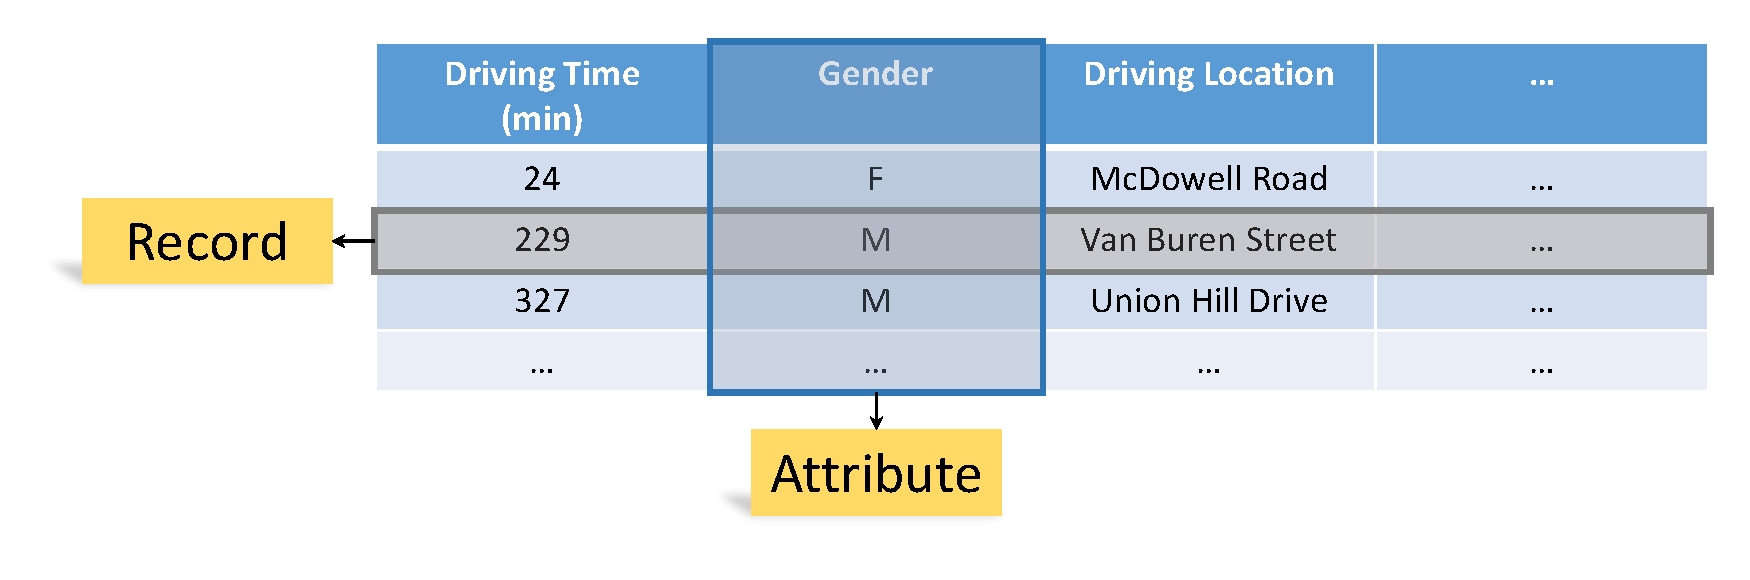
\includegraphics[width=0.9\textwidth]{chapter3/attr_pre}
  %\noindent\rule[0.25\baselineskip]{0.4855\textwidth}{0.95pt}
  \bicaption[fig:attr_pre]{的士司机行车记录数据集}{的士司机行车记录数据集}{Fig}{An illustration of taxi drivers' driving dataset}
\end{figure}

在图\ref{fig:attr_pre}中,我们可以看到该数据集有许多的属性,比如行车时间、司机性别以及行驶地点等等。这些属性的值可以是数值型的,也可以是文字性的。如果数据卖家想基于这些数据的信息量给这个数据集定价,那么其首要问题是弄起初这个数据集含有多少的信息量。因此,我们首要目标是去找到一个合适的方法精确度量该数据集所含有的信息量。在得到了该数据集的信息量之后,我们需要将其映射到一个合适的价格。

用更加形式化的方式叙述上述问题,对于一个有着$m$个属性和$n$条记录的数据集$\bm{D}$,它能表示成一个矩阵$\bm{X}$:
\begin{equation}
\bm{X}=
\left(
\begin{matrix}
 x_{11}      &  x_{12}      & \cdots &  x_{1m}      \\
 x_{21}     &  x_{22}      & \cdots &  x_{2m}      \\
 \vdots & \vdots & \ddots & \vdots \\
  x_{n1}      &  x_{n2}      & \cdots &  x_{nm}      \\
\end{matrix}
\right).
\end{equation}

在矩阵$\bm{X}$中,行向量$\bm{r_i}$表示原数据集中一条记录:
\begin{equation}
\bm{r_i}=\left(
\begin{matrix}
 x_{i1},      &x_{i2},      &\cdots, &x_{im}      \\
\end{matrix}
\right),
\end{equation}

其中,$i=1,...,n$。令$\bm{R}$表示一组记录$\{\bm{r_{i_1}},\bm{r_{i_2}},...,\bm{r_{i_k}}\}$的集合。类似的,列向量$\bm{c_j^\mathrm{T}}$表示原数据集中的一列属性:
\begin{equation}
 \bm{c_j^\mathrm{T}}=\left(
\begin{matrix}
 x_{1j};     &x_{2j};      &\cdots; &x_{nj}      \\
\end{matrix}
\right),
\end{equation}

其中,$j=1,...,m$。同样地,令$\bm{C}$表示一组属性$\{\bm{c_{j_1}},\bm{c_{j_2}},...,\bm{c_{j_k}}\}$的集合。需要指出的是,$\bm{r_i}$中的每个元素的值可以是不同类型的,比如数值、文字、日期等。但是$\bm{c_j}$的元素的值必须是同一类型的。

那么基于信息量的给数据集$\bm{D}$定价的方法可以分为两步:1)量化地度量数据集$\bm{D}$或其子集的信息量$H$;2)基于度量结果,找到一个合适的函数$l(\dot)$,将信息量$H$映射到一个价格$pr$,即$pr=l(H(\bm{D}))$。

为了达到上述目标,在下文中我们首先提出一个基于信息熵的信息量检测方法。然后基于检测结果,我们给出一个定价模型。

\subsection{数据商品信息量的测量}
在本小节中,我们先定义了元组和元组集合。然后,我们基于信息熵\cite{shannon2001mathematical}给出了相应的信息测量方法。

\begin{defn}[元组]
 对于给定的一个数据集$\bm{D}$,元组$\bm{t}$被定义为$\bm{D}$中一条记录$\bm{r}$的非空子集,即$\bm{t} \subseteq \bm{r}$且$\bm{t} \ne \emptyset$。
\end{defn}

\begin{defn}[元组集合]
元组集合$Tup$是一系列元组$\{\bm{t_{i_1}},\bm{t_{i_2}},...,\bm{t_{i_k}}\}$的集合。因此,$Tup$也是数据集$\bm{D}$的非空子集,即$Tup \subseteq \bm{D}$ 且 $Tup \ne \emptyset$。
\label{def:tuple_set}
\end{defn}

对于定义\ref{def:tuple_set},元组集合$Tup$可以是数据集的子集也可以就是数据集本身。实际上,元组集合是本文提出信息测量方法的最小单元。以下四个信息熵测量指标都是基于元组的。

\begin{defn}[数据信息熵]
对于一个有着$n$条元组$\{\bm{t_i}$$|i=1,...,n\}$的元组集合$Tup$,其数据信息熵$H_{ind}$定义为:
\begin{equation}
  H_{ind}(Tup)=-\sum_{\bm{t_i} \in Tup}p(\bm{t_i})\log_{b}p(\bm{t_i}),
  \label{eq:data_individual_entropy}
\end{equation}
\label{def:data_individual_entropy}
\end{defn}
其中,$b$是公式\ref{eq:data_individual_entropy}中对数的基。信息常用度量单位为比特,当对数基底$b$取为$2$时。除非特别指出,下文所有的对数都指的是以$2$为基底的对数,即$\log_2x$。数据信息熵是本文提出数据信息测量方法的最基础概念,它能测量出单个元组集合的信息量。

\begin{defn}[数据联合熵]

对于有$n_1$条元组的元组集合$Tup_1$和有$n_2$条元组的元组集合$Tup_2$,它们的数据联合熵$H_{joint}$定义为:

\begin{equation}\label{eq:joint_entropy}
  \begin{aligned}
    H_{joint}(Tup_1,Tup_2)=-\sum_{\bm{t_i} \in Tup_1} \sum_{\bm{t_j} \in Tup_2} p(\bm{t_i},\bm{t_j}) \log p(\bm{t_i},\bm{t_j})。
  \end{aligned}
\end{equation}

\label{def:data_joint_entropy}
\end{defn}

需要指出的是数据联合熵是可以轻易地扩展到多个元组集合的信息测量。

\begin{defn}[数据条件熵]
对于有$n_1$条元组的元组集合$Tup_1$和有$n_2$条元组的元组集合$Tup_2$,那么在已知$Tup_1$的条件下$Tup_2$的信息熵被定义为
\begin{equation}\label{eq:conditional_entropy}
  \begin{aligned}
    H_{cond}(Tup_2|Tup_1)=-\sum_{\bm{t_i} \in Tup_1} \sum_{\bm{t_j} \in Tup_2} p(\bm{t_i},\bm{t_j})\log p(\bm{t_j}|\bm{t_i}),
  \end{aligned}
\end{equation}
\label{def:data_conditional_entropy}
\end{defn}
其中$H_{cond}(Tup_2|Tup_1)=0$,当且仅当$Tup_2$被$Tup_1$完全决定。换句话说,一旦$Tup_1$已知,$Tup_2$就被唯一确定了。相反的情况是,$H_{cond}(Tup_2|Tup_1)=H_{ind}(Tup_2)$当且仅当$H_{ind}(Tup_1)$和$H_{ind}(Tup_2)$是统计独立的,换句话说就是即使$Tup_1$已知,也不能获得$Tup_2$的任何信息。

\begin{defn}[数据互信息]
对于有$n_1$条元组的元组集合$Tup_1$和有$n_2$条元组的元组集合$Tup_2$,$Tup_1$和$Tup_2$的数据互信息$I$定义为:

\begin{equation}
\label{eq:mutual_information}
  \begin{aligned}
    I(Tup_1;Tup_2)=\sum_{\bm{t_i} \in Tup_1} \sum_{\bm{t_j} \in Tup_2} p(\bm{t_i},\bm{t_j}) \log\frac{p(\bm{t_i},\bm{t_j})}{p(\bm{t_i})p(\bm{t_j})}。
  \end{aligned}
\end{equation}

\label{def:data_mutal_information}
\end{defn}


相比于数据条件熵,数据互信息是被用来度量两个元组的依赖程度。

需要指出的是,元组的元素也可以是连续型数值的。然而上述定义的相关熵都是默认元组元素是离散的。以上定义可以通过将求和符号替换为积分符号后扩展到连续型元组上:

\begin{equation}
  H_{ind}(Tup)=-\int_{\bm{t_i} \in Tup}p(\bm{t_i})\log p(\bm{t_i}),
\end{equation}
\begin{equation}
  H_{joint}(Tup_1,Tup_2)=-\int_{\bm{t_i} \in Tup_1} \int_{\bm{t_j} \in Tup_2} p(\bm{t_i},\bm{t_j}) \log p(\bm{t_i},\bm{t_j}),
\end{equation}
\begin{equation}
  H_{cond}(Tup_2|Tup_1)=-\int_{\bm{t_i} \in Tup_1} \int_{\bm{t_j} \in Tup_2} p(\bm{t_i},\bm{t_j})\log p(\bm{t_j}|\bm{t_i}),
\end{equation}
\begin{equation}
  I(Tup_1;Tup_2)=\int_{\bm{t_i} \in Tup_1} \int_{\bm{t_j} \in Tup_2} p(\bm{t_i},\bm{t_j}) \log\frac{p(\bm{t_i},\bm{t_j})}{p(\bm{t_i})p(\bm{t_j})}.
\end{equation}

然而,对于连续型变量而言,通常是很难确定其概率密度函数。另一方面,在计算机中积分的数值计算也是存在误差的。因此,计算连续型数据的数据信息熵的一般方法是将连续的输入空间切分为若干个离散的子空间,然后按照离散型变量计算其信息熵然。然而这种方法的内部误差会降低计算最后的熵的精确度,那么这就会影响定价策略。对于那些连续型、离散型数据均有的元组,其相应数据信息熵的计算方法是我们未来的工作之一。

此外,\cite{shannon2001mathematical}还列出一系列熵的性质,后续定价函数的讨论涉及到这些性质,因此我们简单陈述下相关性质。

\begin{propt}[数据信息熵的非负性]
\label{pr:entropry_non_negativity}
给定两个元组集合$Tup_1$和$Tup_2$,我们有

\begin{equation}
  H_{ind}(Tup_1)\ge 0, H_{ind}(Tup_2)\ge 0,
\end{equation}
\begin{equation}
  H_{joint}(Tup_1,Tup_2)\ge 0,
\end{equation}
\begin{equation}
  H_{cond}(Tup_1|Tup_2)\ge 0, H_{cond}(Tup_2|Tup_1)\ge 0,
\end{equation}
\begin{equation}
  I(Tup_1;Tup_2)\ge 0.
\end{equation}


性质\ref{pr:entropry_non_negativity}的证明如下:
\begin{proof}
首先来关注数据信息熵,$H_{ind}(Tup)$,其定义如下:

\begin{equation}
    H_{ind}(Tup)=-\sum_{\bm{t_i} \in Tup}p(\bm{t_i})\log p(\bm{t_i})。
    \label{proof:individual_entropy}
\end{equation}

由于 $0\le p(\bm{t_i}) \le 1$,那么

\begin{equation}
\log p(\bm{t_i}) \le 0。
\end{equation}

因此,根据公式(\ref{proof:individual_entropy}), $H_{ind}(Tup)$ 一定是非负的。

$H_{joint}(\cdot)$,$H_{cond}(\cdot)$, $H_{cond}(\cdot)$以及$I(\cdot)$的非负性同样可以采用上述类似步骤证明。

\end{proof}
\end{propt}

\begin{propt}[不同数据信息熵之间的关系]
给定两个元组集合$Tup_1$和$Tup_2$,我们有

\begin{equation}
\label{pr:entropry_relationships}
  H_{joint}(Tup_1,Tup_2)\le H_{ind}(Tup_1)+H_{ind}(Tup_2),
\end{equation}
\begin{equation}
  H_{joint}(Tup_1,Tup_2)\ge H_{ind}(Tup_1),
\end{equation}
\begin{equation}
  H_{joint}(Tup_1,Tup_2)\ge H_{ind}(Tup_2).
\end{equation}

性质\ref{pr:entropry_relationships}的证明如下:
\begin{proof}


首先从数据互信息的定义入手:

\begin{equation}
    I(Tup_1;Tup_2)=\sum_{\bm{t_i} \in Tup_1} \sum_{\bm{t_j} \in Tup_2} p(\bm{t_i},\bm{t_j}) \log\frac{p(\bm{t_i},\bm{t_j})}{p(\bm{t_i})p(\bm{t_j})}.
    \label{app:mutual_information}
\end{equation}


公式(\ref{app:mutual_information})能被重写为:
\begin{equation}
    \begin{aligned}
    I(Tup_1;Tup_2)&=\sum_{\bm{t_i} \in Tup_1} \sum_{\bm{t_j} \in Tup_2} p(\bm{t_i},\bm{t_j}) [\log p(\bm{t_i},\bm{t_j})\\
    &- \log p(\bm{t_i}) - \log p(\bm{t_j})]\\
    &=\sum_{\bm{t_i} \in Tup_1} \sum_{\bm{t_j} \in Tup_2} p(\bm{t_i},\bm{t_j})\log p(\bm{t_i},\bm{t_j})\\
    &-\sum_{\bm{t_i} \in Tup_1} \sum_{\bm{t_j} \in Tup_2} p(\bm{t_i},\bm{t_j})\log p(\bm{t_i})\\
    &-\sum_{\bm{t_i} \in Tup_1} \sum_{\bm{t_j} \in Tup_2} p(\bm{t_i},\bm{t_j})\log p(\bm{t_j}).
    \end{aligned}
    \label{eq:mutal_information_rewrite1}
\end{equation}

根据定义\ref{def:data_individual_entropy}和定义\ref{def:data_joint_entropy},公式~(\ref{eq:mutal_information_rewrite1}) 能进一步写成:

\begin{equation}
\begin{aligned}
    H_{joint}(Tup_1,Tup_2)&=H_{ind}(Tup_1)+H_{ind}(Tup_2)\\
    &-I(Tup_1;Tup_2).
\label{eq:mutal_information_rewrite2}
\end{aligned}
\end{equation}

由于数据信息熵和数据互信息的非负性,我们有:

\begin{equation}
  H_{joint}(Tup_1,Tup_2)\le H_{ind}(Tup_1)+H_{ind}(Tup_2),
\end{equation}

另一方面,根据定义\ref{def:data_individual_entropy},定义\ref{def:data_joint_entropy},以及定义\ref{def:data_conditional_entropy}, 公式(\ref{eq:mutal_information_rewrite1})能进一步写成:
\begin{equation}
    H_{joint}(Tup_1,Tup_2)=H_{cond}(Tup_1|Tup_2)+H_{ind}(Tup_2),
\end{equation}
\begin{equation}
    H_{joint}(Tup_1,Tup_2)=H_{cond}(Tup_2|Tup_1)+H_{ind}(Tup_1).
\end{equation}

类似地,由于数据信息熵的非负性,那么有:

\begin{equation}
  H_{joint}(Tup_1,Tup_2)\ge H_{ind}(Tup_1),
\end{equation}
\begin{equation}
  H_{joint}(Tup_1,Tup_2)\ge H_{ind}(Tup_2).
\end{equation}

\end{proof}
\end{propt}


\subsection{通用定价模型}

在本小节中,我们提出了一个基于数据信息熵的通用定价模型,而不是给出一个具体的定价函数。此外,该定价模型的相关性质和优点在本小节中也会进行讨论。

\begin{defn}[定价函数]
对一个给定的数据集$\bm{D}$,定价函数${pr(\bm{D})}:\bm{D}\to \mathbb{R^{+}}$, 其中 $\mathbb{R^{+}}$ 非负实数。一个基于数据信息熵的定价函数是:
\begin{equation}
  pr(\cdot) \equiv l(H(\cdot)),
  \label{eq:pricing_function}
\end{equation}
其中$l(\cdot)$ 是一个非递减的联系函数,它应该满足如下条件:
\begin{equation}
\forall x_1 \ge x_2, l(x_1) \ge l(x_2),
\label{eq:link_function_property1}
\end{equation}
\begin{equation}
\forall x_1, x_2 \ge 0, l(x_1+x_2) \le l(x_1)+l(x_2).
\label{eq:link_function_property2}
\end{equation}
\end{defn}

\begin{exmp}
对于两个数据集$\bm{D_1}$和$\bm{D_2}$以及一个基于数据信息熵的定价函数$pr(\cdot) \equiv l(H(\cdot))$,如果$H(\bm{D_1})\ge H(\bm{D_2})$,那么有$pr(\bm{D_1})\ge pr(\bm{D_2})$。
\end{exmp}

为了陈述简洁,上述数据信息熵的定价函数都指的是数据独立信息熵或者数据联合熵,取决于$H(\cdot)$中参数个数。选择具体的定价函数要取决于具体的市场情况,这也是本文的未来工作之一。

\begin{propt}[定价函数的非负性]
定价函数的输出一定是大于零的,即$pr(\cdot) \ge 0$总是成立。
\label{pr:pricing_function_pr_1}
\end{propt}

定价函数的非负性是显然的,因为数据卖家在出售商品的同时还倒贴钱给数据买家。接下来,基于数据信息熵的定价函数的\textit{无套利}性质会被讨论,这个性质也是其最大的优点。为了详细地讨论这个性质,我们首先要介绍下一个数据集中的操作,即\textit{连接}。

\begin{defn}[数据集连接]

给定两个数据集$\bm{D_1}$和$\bm{D_2}$,$\bm{D_1}$有$n_1$条记录$\bm{R_1}$和$m_1$条属性$\bm{C_1}$,$\bm{D_2}$有$n_2$条记录$\bm{R_2}$和$m_2$条属性$\bm{C_2}$,$\bm{D_1}$和$\bm{D_2}$的连接$\bm{D_J}$定义为:

\begin{equation}
\bm{D_J}=\bm{D_1} \circledcirc \bm{D_2}.
\end{equation}
\end{defn}

这里给出数据连接操作的两个例子:

\begin{case}
如果在数据集$\bm{D_1}$和$\bm{D_2}$中没有共同的属性,即$\bm{C_1} \cap \bm{C_2} = \emptyset$,那么它们的连接$\bm{D_J}$就会有$n_1+n_2$条记录和$m_1+m_2$条属性。

\end{case}

\begin{case}
如果在数据集$\bm{D_1}$和$\bm{D_2}$中有共同的属性,即$\bm{C_1} \cap \bm{C_2} \ne \emptyset$,那么它们的连接$\bm{D_J}$就会有$n_1+n_2$条记录和$\|\bm{C_1} \cup \bm{C_2}\|$ 条属性。

\end{case}

数据集\textit{连接}的操作能被扩展到多个数据集的情况。如果有多个数据集 $\bm{D_1,D_2,...,D_k}$,我们把他们的连接集合记为$\bm{D_J}=\circledcirc_{i=1}^k \bm{D_i}$。值得注意的是这里的连接操作不同于SQL类的数据库连接操作。为了更加直观地说明这个连接操作,我们举出了如下例子:

\begin{exmp}
数据集$\bm{D_1}$有$3$条记录和$3$个属性$\{a,b,c\}$,数据集$\bm{D_2}$有$4$条记录和$2$个属性$\{c,d\}$。它们的连接数据集$\bm{D_1} \circledcirc \bm{D_2}$将会有$7$条记录和$4$个属性$\{a,b,c,d\}$,如图\ref{fig:joint_data_set}所示。在连接数据集中,那些非共同属性的缺失值是用'\#'填满。
\end{exmp}

\begin{figure}[h]
  \centering
    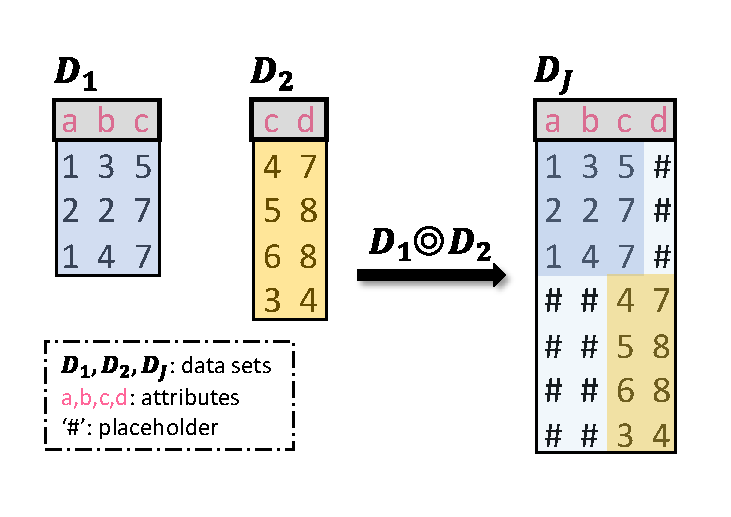
\includegraphics[width=0.7\textwidth]{chapter3/joint_data_set}
  %\noindent\rule[0.25\baselineskip]{0.4855\textwidth}{0.95pt}
  \bicaption[fig:joint_data_set]{数据集连接操作示意图}{数据集连接操作示意图}{Fig}{An illustration of dataset join}
\end{figure}

\subsection{讨论}

\section{实验与评估}

\subsection{实践中遇到的问题}

\subsection{在公开研究数据集上的实验}

\subsection{在大规模工业数据集上的实验}

\subsection{定价函数}

\section{本章小结}
\chapter{基于信息熵的数据商品在线拍卖的研究}

\section{研究动机}
随着近些年人们产生的数据量的巨量增长,关于数据交易的市场雏形可见,并可期成为一个巨大规模的市场。然而,现有的关于传统商品的交易和定价策略是不适用于数据商品的,因为这些交易和定价策略均不能最大化交易双方的总剩余,从而打击交易的积极性和信心。而数据,这一新商品,目前其交易场景多为线上。从而,交易双方的信心和积极性是促成数据交易的关键因素。目前,在这个数据交易市场上,数据买家远多于卖家,使得这个市场近似于一个寡头竞争市场。基于以上两点,我们发现拍卖可能会是一个很好的数据商品定价和交易的机制。一是因为其能最大化交易双方的总剩余,二是因为拍卖机制中本来就有为这种寡头竞争市场专门设计的规则。但这不意味着我们可以直接把为传统商品设计的拍卖机制直接应用到数据商品上,因为数据商品和传统商品有很大的区别。相比于传统商品,数据商品具有唯一性和不确定均衡价格。

在众多关于拍卖的研究文献中\cite{Vickrey1961Counterspeculation,Milgrom1989Auctions,Milgrom1982A,Riley1981Optimal},拍卖物的价值$v$被认为是服从一个均匀分布,即$v\sim U[v_l,v_h]$,其中$v_l$是估价的下限,$v_h$是估价的上限。但是这些文献均没有给出如何估计上下限的指导方法,而估值上下限却是实施拍卖机制的基础。相比于传统商品,数据商品更无形,更加抽象,因此更难以被普通消费者估计它们的价值。尽管现在已经有一些关于数据商品的评价指标,比如数据集大小,数据集生成时间等,但这仍是远远不够的。我们需要找一个更合适的指标来评估数据集,从而指导拍卖参与者对数据商品的估价。目前,Li等人\cite{li2017first}提出了数据信息熵这一新的指标,用来测定给定数据集的信息量和清晰地描述数据集内的信息分布,在他们文中还提出了一系列基于该指标定价的好处。数据信息熵可能是一个非常合适的帮助数据商品估价的指标,我们期望先用数据信息熵测定给定数据商品的信息量,然后基于它给出该商品的估值上下限,从而实施拍卖机制。

\section{影响在线拍卖的重要因素}
文献\cite{Pinker2003Managing}提出了一些影响在线拍卖的重要因素,但是没有真实拍卖交易数据的支持。因此,我们收集了2012年12月到2013年eBay Live Auction的一些交易记录,希望以此佐证文献\cite{Pinker2003Managing}提出的这些影响因素。这些数据集包含了Cartier手表,Palm Pilot M515掌上智能机,Xbox游戏终端以及Swarovski珍珠项链在这段时期的相关拍卖信息。具体来说,它包含了相关的九个变量,即拍卖入场时间,拍卖持续时长,成交价等。在这个数据集中,总共有三种类型的拍卖,分别是时长为3天的拍卖,时长为5天的拍卖和时长为7天的拍卖。为了能挖掘拍卖价格,入场时间以及拍卖持续时长的关系,我们将该数据集中部分记录进行了可视化,如图\ref{fig:number of bidders distribution histogram}。这些可视化帮助我们更加清晰地认知这些因素是如何影响拍卖的。以下是我们在设计数据商品在线拍卖模型时最关心的三个因素。

\subsection{拍卖机制}

第一价格拍卖、第二价格拍卖、英式增价拍卖、荷兰式减价拍卖是目前用的最多也是被研究的最多的四种拍卖机制。其中,英式增价拍卖在在线网络拍卖中是用得最多的,因为它是顾客最熟悉、接触最多的拍卖机制。目前,最大的在线拍卖网站,eBay Live Auction 采用的正是英式拍卖。eBay Live Auction已成功吸引了数以百万计的人参与他们的在线拍卖,这从侧面佐证了英式增价拍卖的可用性。

然而, Milgrom等人\cite{Milgrom1989Auctions}提出英式拍卖机制容易受到不同欺诈行为的影响。Pinker等人\cite{Pinker2001Using,Pinker2003Managing}认为一个好的拍卖机制必须居然三个特指:1)对不同顾客行为鲁棒的;2)分配是要高效的;3)要能有效应对欺诈行为的。设计一个最优拍卖仅仅是存在于理论中的,因为最优拍卖机制中的许多假设在现实中是难以满足的。另外,理论上的最优拍卖机制在市场中是难以实现的。Myerson\cite{Myerson1981Optimal}在上述四个拍卖机制下提出了收益均衡定理。Lucking-Reiley\cite{Lucking1999Using}通过对邮票的在线拍卖的实验,比较了英式拍卖和第二价格拍卖的收入产生。他们的目标是去验证Myerson的收益等价定理在英式拍卖和第二价格拍卖下是否成立。他们发现,这二者的最终收益的差别是非常小的,因此我们也认为在线英式拍卖的理论经验是可靠的。

大量关于在线拍卖的研究是集中在前向拍卖 (forward auction), 即是一个卖家向多个买家拍卖物品。以上提到的四个拍卖机制均是前向拍卖。然而,还是存在另外一大类拍卖,反向拍卖 (reverse auction),即一个买家需要买一件物品,多个卖家以竞争的方式提供该物品,这个场景多出现在政府项目招标中。然而,对于数据的在线拍卖,是不太适合使用反向拍卖作为拍卖机制的,因为目前市场上并没有足够多的数据提供商去满足众多数据买家的需求。

\subsection{竞拍时长与参与人数}
\label{subsec:auction duration and bidder number}
竞拍时长在在线拍卖中有着很大的作用。相比于传统的只持续数十分钟或数个小时的传统公开拍卖,在线拍卖往往会持续数天或数周。因为在线拍卖不会要求竞拍人到场,他们能在任何地点任何时间参与拍卖\cite{Pinker2003Managing}。因此,持续时间很长的在线拍卖是可行的。传统拍卖往往会以一个固定的竞拍人数开始拍卖,而相应的关于期望收益和最优保留价的分析都是基于这固定的竞拍人数的。但是,同样的分析方法就不适用于在线拍卖。因为,在网络上,在线拍卖的人数是不固定的,而在线拍卖的竞拍人数往往是由竞拍时长决定的。

\begin{figure}
   \centering
   \subfigure[持续时长为3天的拍卖]{
     \label{fig:3-day auction} %% label for first subfigure
     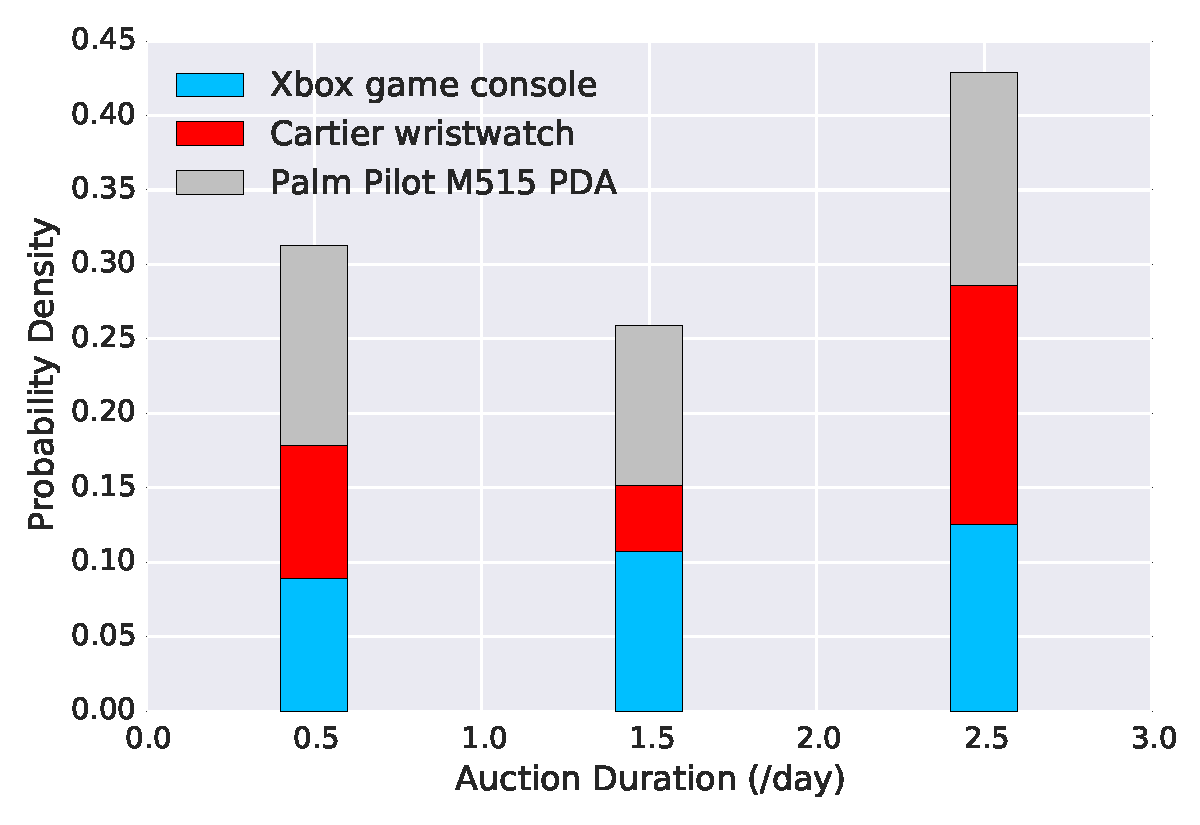
\includegraphics[width=0.55\textwidth]{chapter4/3_days_hist}}
   \subfigure[持续时长为5天的拍卖]{
     \label{fig:5-day auction} %% label for second subfigure
     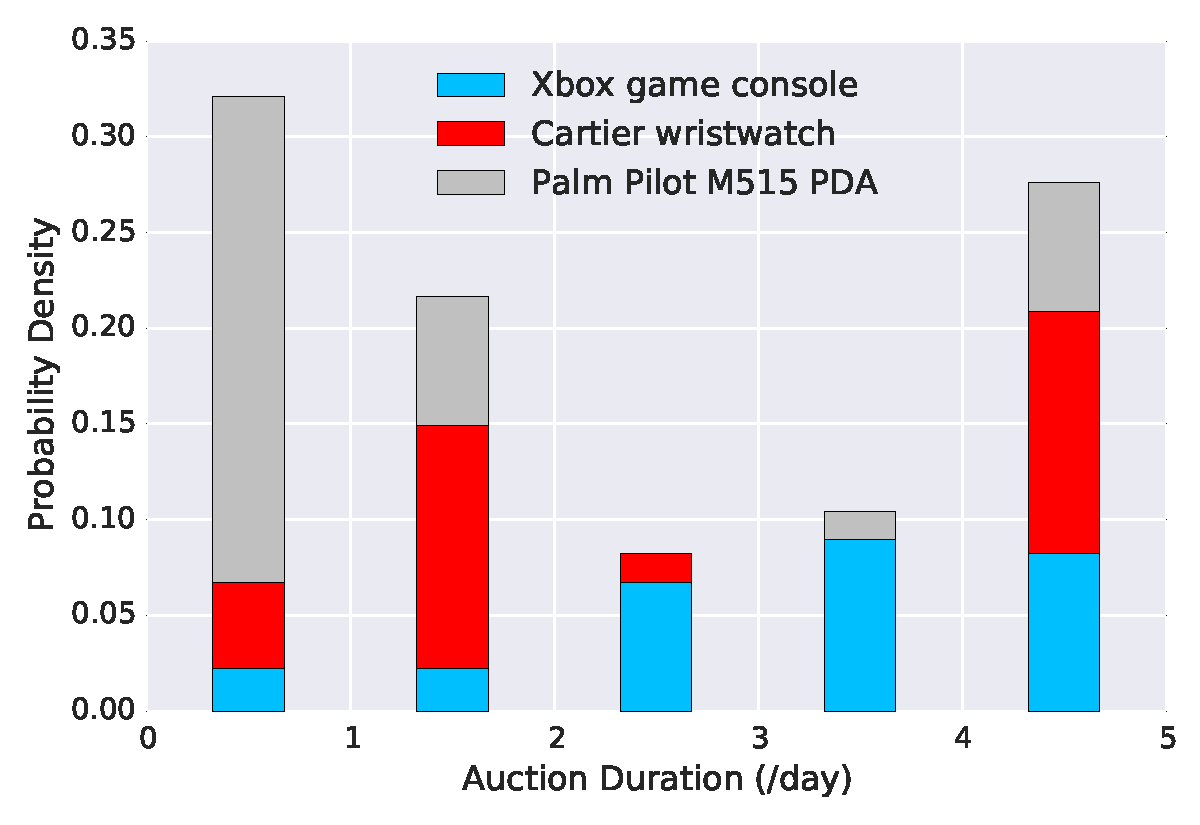
\includegraphics[width=0.55\textwidth]{chapter4/5_days_hist}}
   \subfigure[持续时长为7天的拍卖]{
     \label{fig:7-day auction} %% label for second subfigure
     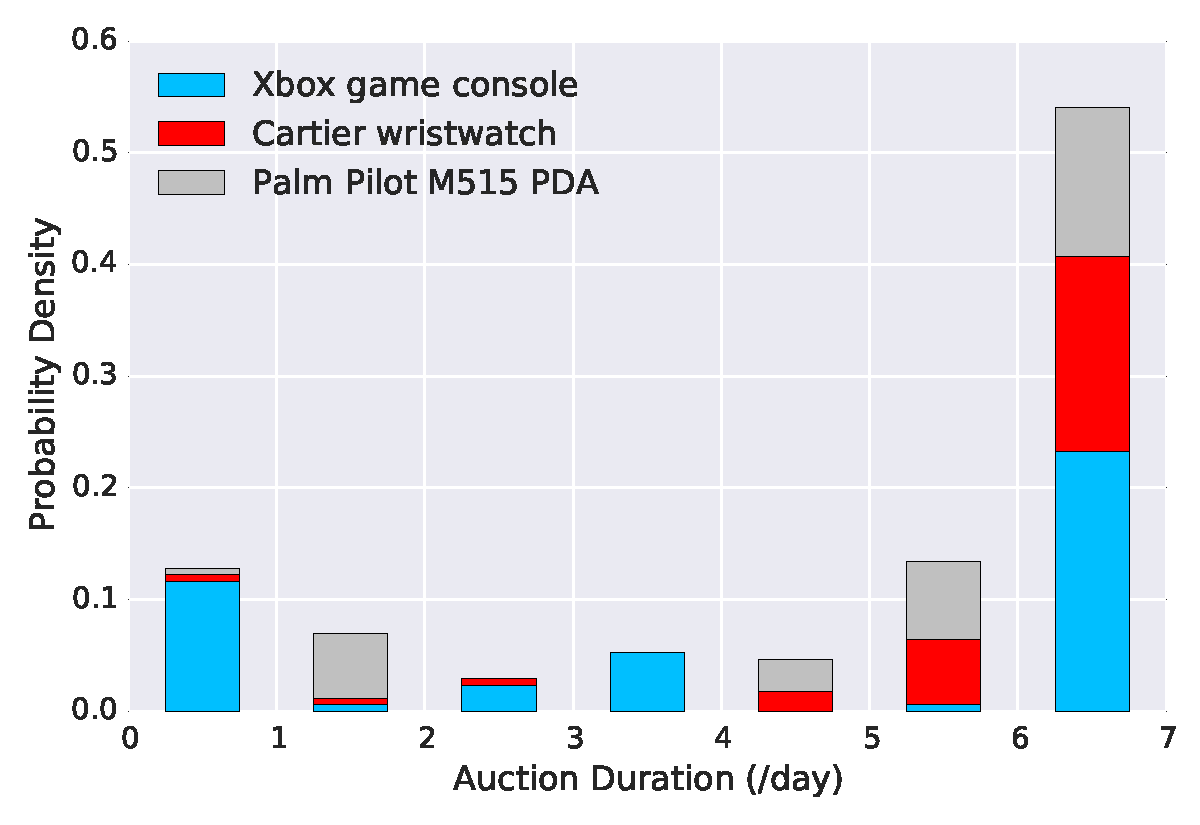
\includegraphics[width=0.55\textwidth]{chapter4/7_days_hist}}
   \bicaption[fig:number of bidders distribution histogram]{竞拍参与人数分布直方图}{竞拍参与人数分布直方图}{Fig}{Number of bidders distribution histogram}
 \end{figure}

目前,在在线拍卖市场上有两大类方法终止拍卖,分别是硬结束时间 (hard deadline) 和软结束时间 ("going, going, gone")。前一个,硬结束时间被eBay Live Auction采用:超过了硬结束时间的竞拍是不被接受的。后者,软结束时间被Amazon Auction使用\cite{amazonauction},在Amazon的在线拍卖市场上,拍卖持续时间会被自动延长只要在结束时间之前有新的竞拍。Roth和Ockenfels\cite{Roth2002Last}发现延迟竞拍 (late bidding) 和狙击竞拍 (snipe bidding) 时常发生在硬结束时间的在线拍卖中,比如eBay Live Auction。我们从eBay Live Auction收集到的真实买拍数据中也发现了这个现象。图\ref{fig:number of bidders distribution histogram}是在三种不同持续时长下的三种不同物品的在线拍卖。可以从这三幅子图中看出,竞拍者大多数会“挤”在拍卖的最后一天参与拍卖。Pinker\cite{Pinker2003Managing}称当在线拍卖网站流量很低的时候,延长拍卖在一定程度上可能有助于提高成交价。然后,这并不意味着可以一味地延长拍卖时间。Ariely等人\cite{Dan2003Buying}却认为即使更短的拍卖持续时间可能会只吸引更少的竞拍者,但是这样能增加竞拍者之间的竞争激烈度。他们在自己的实验中记录到拍卖时长是与成交价呈负相关关系。在本文中,为了更好地对在线拍卖竞拍者参与过程进行动态建模,我们将竞拍人数考虑成为拍卖持续时间的分段函数。

\subsection{起拍价与保留价}

起拍价可以理解成为另一种形式的保留价,通常是要么公开,要么保密。起拍价迫使竞拍者需要竞拍时高于起拍价。而保留价是拍卖者为成交价设定的一个下限。如果竞拍结束时,最高竞拍价还低于保留价的话,那么卖家有权利撤销这次拍卖。

从大量的拍卖记录中,我们发现如果竞拍者人数不够的话,那么最终成交价就会比较低。而竞拍者人数不仅仅与竞拍持续时间也与起拍价相关。Vakrat等人\cite{Pinker2001Using}经过分析实例发现当没有起拍价限制时,拍卖品会以低于相应零售商给出的价格很多的成交价被拍出。当起拍价增加时,成交价很大可能会趋近于起拍价。如果起拍价进一步增加,拍卖流拍的可能性会骤增。Reiley等人\cite{Ockenfels2006Online}发现设置了公开的起拍价和保留价后会减少竞拍人数,并且也会增加拍卖品流拍的可能性。同样地,Ariely等人\cite{Dan2003Buying}发现了起拍价和成交价之间具有正相关关系。即使一个很低的起拍价会吸引更多的竞拍者,但是竞拍者的出价会很低,不足以在拍卖者之间产生价格竞争。此外,通过大量的实例调查,Bradlow等人\cite{Bradlow2007Bayesian}发现起拍价与竞拍时间的增幅是具有负相关关系的。这也意味着一个低的起拍价会在短时间吸引更多的竞拍者。在本文提出的在线拍卖模型中,我们将起拍价就认为是保留价,以期望去探索发现保留价和卖家期望收益的关系。

\section{基于信息熵的在线拍卖模型}
在本小节中,我将陈述基于信息熵的在线拍卖模型。首先,用$\lambda_t$表示在线拍卖开始时间t后单位时间内的竞拍者到达率。值得指出的是,$\lambda_t$是与许多因素相关的,比如拍卖持续时间、当前参与拍卖人数、当前最高价以及竞拍规则。当然,肯定还有其他因素影响着在线拍卖。在真实情况中,在时间段$[t,t+\delta t]$内到达的竞拍者人数是一个随机变量。Vakrat和Seidmann\cite{Vakrat2000Implications}发现在线拍卖中新竞拍者的到达过程与指数分布非常相似。为了简化竞拍者的到达过程,同时也为了更好的抓住在线拍卖的动态特征,Chen等人\cite{Chen2007Optimal}将在线拍卖的竞拍者到达过程拟合成了一个泊松分布。该泊松分布的参数设为$\lambda$,可认为是在线拍卖中的竞拍者到达率。具体的,$N$个竞拍者在时间长度$t$内到达的概率质量函数被定义为:
\begin{equation}
\label{eq:number of bidder}
P_t(N=n)=\frac{e^{-\lambda t}(\lambda t)^n}{n!},n=0,1,2,...
\end{equation}

然而,在实际的在线拍卖中,到达率$\lambda$并不会全程保持不变。我们可以从图\ref{fig:number of bidders distribution histogram}发现到达率$\lambda_t$在在线拍卖过程中是变化的。为了比Chen等人提出的模型更好地抓住在线拍卖的动态特征,我们将拍卖持续时长$[0,T]$切分为一组不重叠的子区间,以使得到达率$\lambda_t$在不同子区间内取不同的值,然而在子区间内保持不变。

在我们的模型中,在线市场的数据卖家会列出他们要出售数据商品$D$的一些指标,去帮助买家估计该商品的价值。这些指标有$H(D)$,数据信息熵\cite{li2017first};$s(D)$,数据集的大小;或者是数据集的生成时间等等。每一个潜在竞拍者都会在参加拍卖前浏览这些信息。利用这些信息,潜在的拍卖者可以给待拍卖的商品估计出一个价值区间$[v_l,v_h]$。因为,本文主要关注基于信息熵的在线拍卖,我们将这一估计过程定义为如下:
\begin{equation}
\label{eq:v_l}
%v_l=\frac{H(x)}{s(x)},
v_l \propto H(D),
\end{equation}
\begin{equation}
\label{eq:v_h}
v_h \propto\alpha H(D),\alpha\ge 1,
%v_h=\alpha\frac{H(x)}{s(x)},\alpha\ge 1,
\end{equation}

其中,$\alpha$是放大系数。

在在线拍卖中,我们用元组$(a_i,b_i)$分别表示竞拍者$i$的到达时刻和出价。出价$b_i$是与拍品的真实价值$v_i \in [v_l,v_h]$相关的,记为$b_i=b(v_i)$。如果在时刻$t$有$n_t$个竞拍者参与当次拍卖,对于当前时刻$t$,我们将这些竞拍者记为一个集合$B$。在这个集合中,对于所有的竞拍者,其到达时间$a_i \le t, i=1,2,...,n_t$。这些竞拍者的出价构成一个出价向量$\vec{b}_t=(b_1,b_2,...,b_{n_t})$。

现在我们已经为时刻$t$的在线拍卖定义了两个状态变量$n_t$和$\vec{b}_t$。如果此次拍卖中有$k$个物品要拍卖。那么在拍卖的结尾时,那么将会有一个成交价向量$\vec{p}=(p_1,p_2,...,p_k)$。这个成交价向量是竞拍总人数$n_T$,竞拍出价向量$\vec{b}_T$,状态变量的最终值以及拍卖规则$\textbf{R}$的函数。对于卖家而言,他的目标是最大化拍卖物品的成交价,即:

\begin{equation}
\max_{\textbf{R},T} \arrowvert \vec{p}(n_T,\vec{b}_T) \arrowvert_1,
\end{equation}

其中$\arrowvert\cdot\arrowvert_1$是向量的$L_1$范数。拍卖规则$\textbf{R}$规定着1)拍卖结束时商品是如何分配的;2)成交价是如何决定的;3)出价是公开还是密封的;4)是否有保留价;5)保留价是公开的还是密封的等等\cite{Pinker2003Managing}.。假设卖家为每一个竞拍者设计一个估价区间$V_i=[v_l,v_h]$。令$V=\prod_{i=1}^{n}V_i$,表示所有竞拍者联合估价。除此以外卖家还需要设计分配规则$q(v)$对于每一个联合估价$v \in V$。具体来说,$q(v)=(q_1(v),q_2(v),...,q_n(v))$是一个概率向量,其中$q_i(v)$是第$i$个竞拍者赢得拍品的概率。此外,本文还定义了一个支付向量$p(v)=(p_1(v),p_2(v),...,p_n(v))$,其中$p_i(v)\in \mathbb{R}$是第$i$个竞拍者期望支付价格。因为参加拍卖是自愿的,我们假设对于每个竞拍者$i$,如果他的估价低于卖家的最低价,那么他会选择不参加此次竞拍,即$np \in V_i$。具体来说,如果$v\in V$并且$v_i=np$, 那么 $p_i(v)=0$且$q_i(v)=0$。

现如今,英式拍卖,荷兰式拍卖,第一价格拍卖以及第二价格拍卖是最普遍也是被研究地最多的四种拍卖机制。尤其是英式拍卖如今最流行的。在开始陈述本文提出的模型之前,需要作出以下假设:

\begin{assmp}[个人估价私密性]
\label{conj:private value}
  对于竞拍者$i$,他对拍卖品的估价$v_i$是只有他自己知道的,卖家和其他竞拍者是不清楚的。但是所有拍卖参与者都默认$v_i$是一个落在区间$[v_l,v_h]$的随机变量,还知道其概率分布函数$F_i(v_i)=\int_{v_l}^{v_i}f_i(z)dz$,其中$f_i$是严格大于零的连续密度函数。
 
\end{assmp}

\begin{assmp}[估价的独立性]
\label{conj:independent value}
  简单来说,每个竞拍者的估价$v_1,v_2,...,v_n$是独立的,也就是说$v_1,v_2,...,v_n$的联合概率分布函数为
  \begin{equation}
	F(v_1,v_2,...,v_n)=F_1(v_1)F_2(v_2)...F_n(v_n).
	\end{equation}
 
\end{assmp}

\begin{assmp}[估价分布函数的对称性]
\label{conj:symmetric distribution function}
这些概率分布函数是相同的,对于所有的$i,j=1,2,...,n$ 和 $v\in[v_l,v_h]$,有
	\begin{equation}
	F_i(v)=F_j(v)=F(v).
	\end{equation}
 
\end{assmp}

\begin{assmp}[竞拍者风险中立]
\label{conj:risk nuetral}
对于每个竞拍者,他的目标是最大化其期望收益。
 
\end{assmp}

\begin{assmp}[无串通性]
\label{conj:no collusion}
每一个竞拍者都是独立地决定其竞拍策略,在竞拍者之间没有串通。
\end{assmp}

不同于传统拍卖,在线拍卖并不需要召集所有的参与者到拍卖行中。因此,在线拍卖的竞拍者之间串通的可能性是远远小于传统拍卖的。

以上所有假设描述了对称独立私有价值条件(Symmeteric Independent Private Value, SIPV)。对于卖家来说,Meyerson\cite{Myerson1981Optimal}发现了在前面提到过的四种拍卖机制下收益是等价的。由于收益等价定理,在某种程度上来说,以上四种拍卖机制是等价的。本文选择在对称独立私有价值条件下的第二价格拍卖作为在线拍卖机制。为不失一般性,本文将第二价格拍卖扩招到适用于$k$物品的第$k$价格拍卖。本文形式化地将对于数据商品的在线第$k$价格拍卖描述在算法xx中。



\subsection{带保留价的单件物品在线拍卖}

在本小节中,我们先讨论设置了公开保留价的单件商品的在线拍卖,也就是这里的$k=1$。在传统的第二价格拍卖中,Riley和Samuelson\cite{Riley1981Optimal}得出了这样的结论:当对称独立私有价值条件满足时,对于设置了合适的保留价$r$和有$n$个竞拍者的在线拍卖,卖家的期望收益为:
\begin{equation}
\label{eq:basic expected revenue}
R_s=n\int_{r}^{v_h}(xf(x)+F(x)-1)F^{(n-1)}(x)dx.
\end{equation}

在单件商品在线拍卖中,数据卖家只卖出一件数据商品。因为在在线拍卖中,竞拍者人数$N$也是一个随机变量,卖家的期望收益应当是与$N$有关的,即:

\begin{equation}
\label{eq:basic online expected revenue}
R_s^{online}=E_N(R_s).
\end{equation}

Chen等人\cite{Chen2007Optimal}将竞拍者参与在线拍卖的过程建模为一个到达率为常量$\lambda$的泊松过程。本文提出的在线拍卖模型也是一个泊松过程,但是该到达率是在不同时段是变化的。我之所以这样建模是基于对eBay Live Auction拍卖数据记录的观察,在小节\ref{subsec:auction duration and bidder number}中描述了竞拍者在竞拍过程中的到达率是不一样的,一般是初期的到达率很高,中期到达率比较低,然后到竞拍快结束时达到最高峰。因此,我们将整个竞拍时长$[0,T]$划分为$M$个不重叠的子区域$\{I_i\}_{i=1}^M$,其中$I_i=[t_{i-1},t_i]$。在不同的子区间中,到达率$\lambda$取不同的值 $\{\lambda_1,\lambda_2,...,\lambda_M\}$,但在子区间内到达率保持不变。因此,对于一个在时间区间$I_i=[t_{i-1},t_i]$保留价为$r$的在线拍卖而言,有$n_i$个人参与的概率为:
\begin{equation}
\label{eq:Ni}
P(N_i=n_i|\lambda_i)=\frac{e^{-z_i}z_i^{n_i}}{n_i!},
\end{equation}
其中,$z_i=\lambda_i(t_i-t_{i-1})(1-F(r))$,$N_i$是在时间区间$I_i=[t_{i-1},t_i]$内参与拍卖的人数。为了易于建模,在本文中假设不同区间内的到达率$\lambda_i$是相互独立的。但是,在实际中,不同区间的竞拍者到达率却是与其前一个到达率和当前最高出价$b^*$相关的。对于竞拍者到达过程更加精确的建模是本文未来的工作之一。那么,总共有$N$个竞拍者参与此次拍卖的概率为:
\begin{equation}
\label{eq:N}
P(N=n_1+n_2+...+n_M|\vec{\lambda})=\prod_{i=1}^{M}P(N_i=n_i|\lambda_i),
\end{equation}
其中$\vec{\lambda}$是参数向量$(\lambda_1,\lambda_2,...,\lambda_M)$。在所有$(n_1,n_2,...,n_M)$可能取值上的$P(N=n_1+n_2+...+n_M|\vec{\lambda})$的和完全定义了在时间段$[0,T]$上有$N$个人的概率空间。此外,参数向量$\vec{\lambda}$是取决于时间段$[0,T]$的划分的。一旦确定了时间段的划分规则,我们就能使用极大似然估计\cite{Bock1982Marginal,Zhou2017An}从之前收集到的拍卖数据估计出$\vec{\lambda}$。

在数据卖家出售其数据商品之前,他还有收集和清理数据商品的固定成本。我们将这一成本定义为$c$。基于公式(\ref{eq:basic expected revenue}) (\ref{eq:basic online expected revenue}) (\ref{eq:Ni})以及(\ref{eq:N}),本文为在线第二价格拍卖定义了以下的卖家期望收益:

\begin{defn}[卖家期望收益]
 \label{seller revenue defintion}
	假设对称独立私有价值条件被满足,且卖家设置了保留价$r$,其固定成本为$c$,那么对于该卖家的期望收益为:

	\begin{equation}
	\label{eq:single item expected revenue}
	\begin{aligned}
	R_{s}^{online}&=E_N(R_s|\vec{\lambda})-c\\
	&=\sum_{n_1=0}^{\infty}\sum_{n_2=0}^{\infty}...\sum_{n_M=0}^{\infty}\prod_{i=1}^{M}P(N_i=n_i|\lambda_i)R_s-c.
%	&=\sum_{n=0}^{\infty}P_T(N=n)R_s-c\\
%	&=\sum_{n=0}^{\infty}\frac{e^{-z}z^n}{n!}R_s-c\\
%	&=\sum_{n=0}^{\infty}\frac{e^{-z}z^n}{(n-1)!}\int_{r}^{v_h}[xf(x)\\
%	&+F(x)-1)]F^{(n-1)}(x)dx-c,
	%&=\sum_{n=0}^{\infty}\frac{e^{-z}z^n}{n!}v_0F^n(r)-c+\\
	%&\sum_{n=0}^{\infty}\frac{e^{-z}z^n}{n!}n\int_{r}^{v_h}(xf(x)+F(x)-1)F^{(n-1)}(x)dx
	%&=v_0exp[\lambda t(1-F(r))^2]+\\
	%&\lambda t\int_{r}^{v_h}[F(x)+xf(x)-1]exp[-\lambda t(1-F(r)(1-F(x))]dx
	\end{aligned}
	\end{equation}

需要强调的是$R_s$中的$n$是被$n_1+n_2+...+n_M$替换的。
\end{defn}

\begin{prop}
\label{proposition1}
对于在线第二价格拍卖,如果对称独立私有价值条件被满足,卖家的最优保留价为:
\begin{equation}
	\label{eq:optimal reserve price}
	r^*=\frac{1-F(r^*)}{f(r^*)},
\end{equation}

这样,卖家就能获得最大的期望收益。此外,观察上式可以发现最优保留价$r^*$是独立于竞拍者人数的。
\end{prop}

根据Vickrey的洞见\cite{Vickrey1961Counterspeculation},竞拍者在第二价格拍卖中的最优竞拍策略就是尽可能地出他的真实估价,即$b_i(v_i)=v_i$。那些出价最高的竞拍者赢得商品,他们需要支付$p_i(v)$。在单件商品第二价格拍卖中,竞拍获胜者只有一位。因此,竞拍获胜者支付价格为$b^*_2(v)$,即该次拍卖中的第二高竞拍价。由于$b_i(v_i)=v_i$,因此$b^*_2(v)=v^{(2)}$。而$v^{(2)}$也是一个随机变量,其概率密度函数\cite{Riley1981Optimal}定义为:
\begin{equation}
p(v^{(2)})=n(n-1)f(v^{(2)})F^{(n-2)}(v^{(2)})[1-F(v^{(2)})].
\end{equation}

\begin{defn}[竞拍胜者支付价格]
	\label{winning price definition}
	假设对称独立私有价值条件被满足,竞拍胜者的期望支付价格$v^{(2)}$定义为:
	\begin{equation}
	E(v^{(2)})=\sum_{n_1=0}^{\infty}\sum_{n_2=0}^{\infty}...\sum_{n_M=0}^{\infty}\prod_{i=1}^{M}P(N_i=n_i|\lambda_i)\int_{r}^{v_h}p(x)dx.
	%\sum_{n=0}^{\infty}P_T(n) \int_{r}^{v_h}n(n-1)f(x)F^{(n-2)}(x)[1-F(x)]xdx\\
	%&=\sum_{n=0}^{\infty}\frac{e^{-z}z^n}{(n-2)!}\int_{r}^{v_h}f(x)F^{n-2}(x)[1-F(x)]xdx.
	\end{equation}
\end{defn}

$E(v^{(2)})$也是拍卖物品的最后成交价,它也可以被视为数据商品$D$的定价函数$pr(\dot)$。Li\cite{li2017first}等人讨论了基于数据信息上的定价函数需要满足什么样的条件能使得该函数是无套利的。在本文中,我将$E(v^{(2)})$视为与数据信息熵$H$的联系函数因为根据公式(\ref{eq:v_l})和(\ref{eq:v_h})。

\begin{prop}
\label{proposition2}
	期望成交价$E(v^{(2)})$是无套利的, 如果 1) $E(v^{(2)})$ 是凹函数; 2) 放大系数满足如下公式:
	\begin{equation}
		\frac{f(\alpha H)[1-F(\alpha H)]}{f(H)[1-F(H)]} \ge 1. 
	\end{equation}
\end{prop}

在实际中,放大系数$\alpha$是取决于竞拍者对于数据商品价值的主观估计,所以$\alpha$也是一个随机变量。该变量能帮助我们判断基于信息熵的在线拍卖无套利的概率,如何估计这一概率是我们未来的工作之一。

\subsection{带保留价的多件物品在线拍卖}
在多件物品的在线拍卖中,数据卖家会以一个公开的保留价$r$出售$k$件相同的数据商品。假设在拍卖进行的时刻$T$有$N$个风险中立的竞拍者参与进来,并且每一个竞拍者只想拍一件商品。在多件物品在线拍卖中,我们采用第$k$价格拍卖规则,其中竞拍获胜者是出价前$k$高的人,他们只需支付第$k+1$高的出价来获得拍品,第$k+1$高的出价记为$b^{(k+1)}$(从另一个角度来说,这也是最低竞拍获胜价格)。而对于竞拍者来说,他们的最优竞拍策略仍是出他们的真实估价,即$b_i(v_i)=v_i$. 因此, $b^{(k+1)}=v^{(k+1)}$。

下面,我们讨论$v^{(k+1)}$的期望着。假设已有$n>k$个人竞拍者参与拍卖。那么其中$k$个竞拍者出价高于或等于$v^{(k+1)}$,剩下$n-k$个竞拍者出价低于$v^{(k+1)}$的概率是$C^{k}_{n}F^{(n-k)}(v^{(k+1)})[1-F(v^{(k+1)})]^k$。那么,$v^{(k+1)}$的期望值为:
\begin{equation}
\begin{aligned}
	E(v^{(k+1)}) =&\int_{r}^{v_h}\frac{n!}{k!(n-k)!}F^{(n-k)}(v^{(k+1)})\\
&[1-F(v^{(k+1)})]^kf(v)vdv.
\end{aligned}
\end{equation}
其中竞拍人数$N$是一个随机变量,因此$v^{(k+1)}$对于拍卖人数$N$的期望为:
\begin{equation}
E_N(v^{(k+1)}|\vec{\lambda}) = \sum_{n_1=0}^{\infty}\sum_{n_2=0}^{\infty}...\sum_{n_M=0}^{\infty}\prod_{i=1}^{M}P(N_i=n_i|\lambda_i)E(v^{(k+1)}).
\end{equation}

$E_N(v^{(k+1)}|\vec{\lambda})$为这$k$件商品的最终成交价。如果卖家的固定成本$c$被计算在内的话,那么卖家的期望收益是 $kE_N(v^{(k+1)}|\vec{\lambda})-c$,即:
\begin{equation}
R_{s,k}^{online} = k(E_N(v^{(k+1)}|\vec{\lambda})-c).
\end{equation}

\section{模型评估}

在本小节中,我们为本文提出的一系列定义和命题给出可视化的数值结果。

\subsection{卖家期望收益与保留价的关系}

在前文中,我们已经定义了卖家的期望收益$R_s^{online}$和相应的最优保留价$r$。我们将通过观察$R_s^{online}$随保留价$r$的变化趋势来验证我们提出的卖家期望收益$R_s^{online}$和最优保留价$r$的合理性。这里,精确的$R_s^{online}$是根据公式(\ref{eq:single item expected revenue})求得。为了简化计算,我们将公式(\ref{eq:basic online expected revenue})中的多阶段泊松过程简化成了一阶段泊松过程以此来计算了近似的$R_s^{online}$,即:
\begin{equation}
\label{eq:simplified online expected revenue}
\begin{aligned}
R_s^{online}=\lambda T \int_{r}^{v_h} [F(x)+xf(x)-1]\exp[-\lambda T(1-F(r))(1-F(x))]dx.
\end{aligned}
\end{equation}

\begin{figure}[b]
	\centering
	\subfigure[$T=3,v_l=10,v_h=100$]{
		\label{fig:T=3vl=10vh=100}
		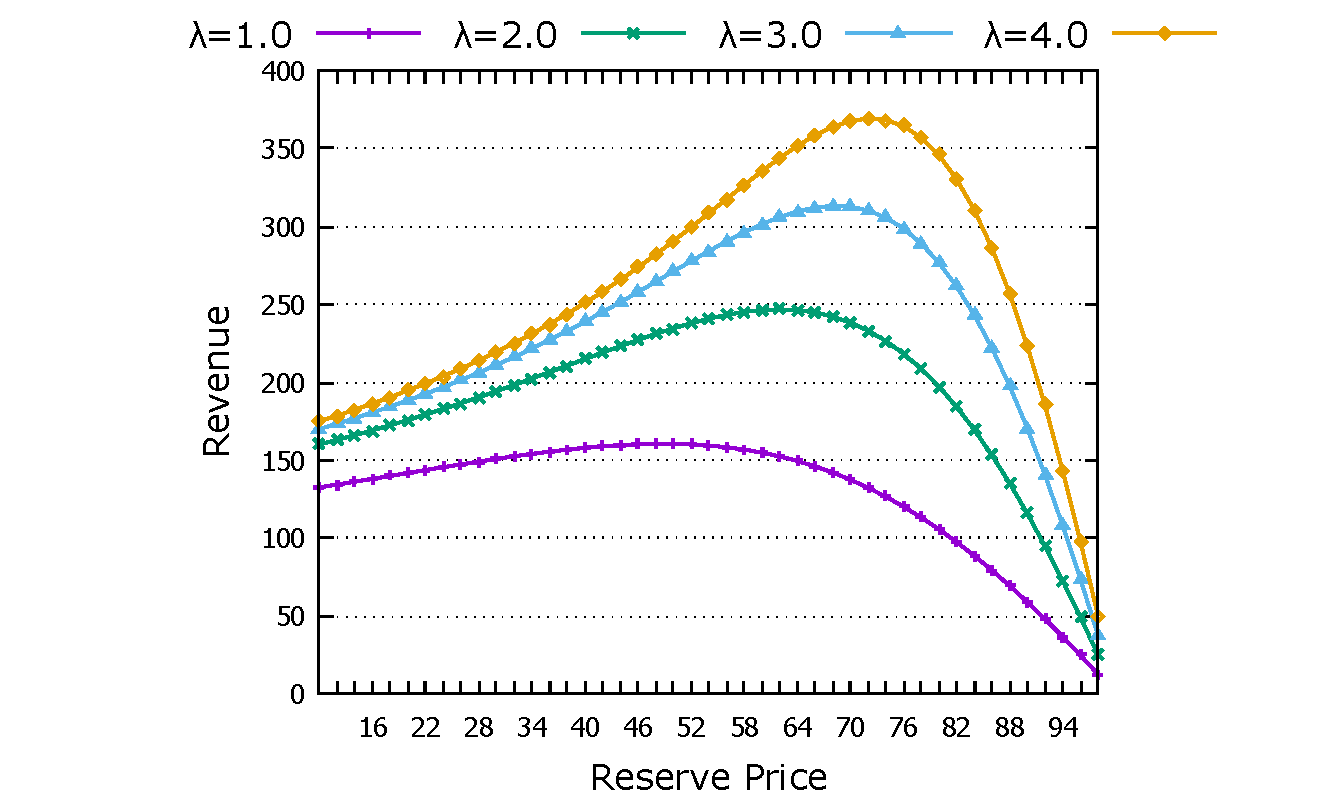
\includegraphics[width=0.4\textwidth]{chapter4/T=3vl=10vh=100.pdf}
	}
	\subfigure[$T=5,v_l=10,v_h=100$]{
		\label{fig:T=5vl=10vh=100}
		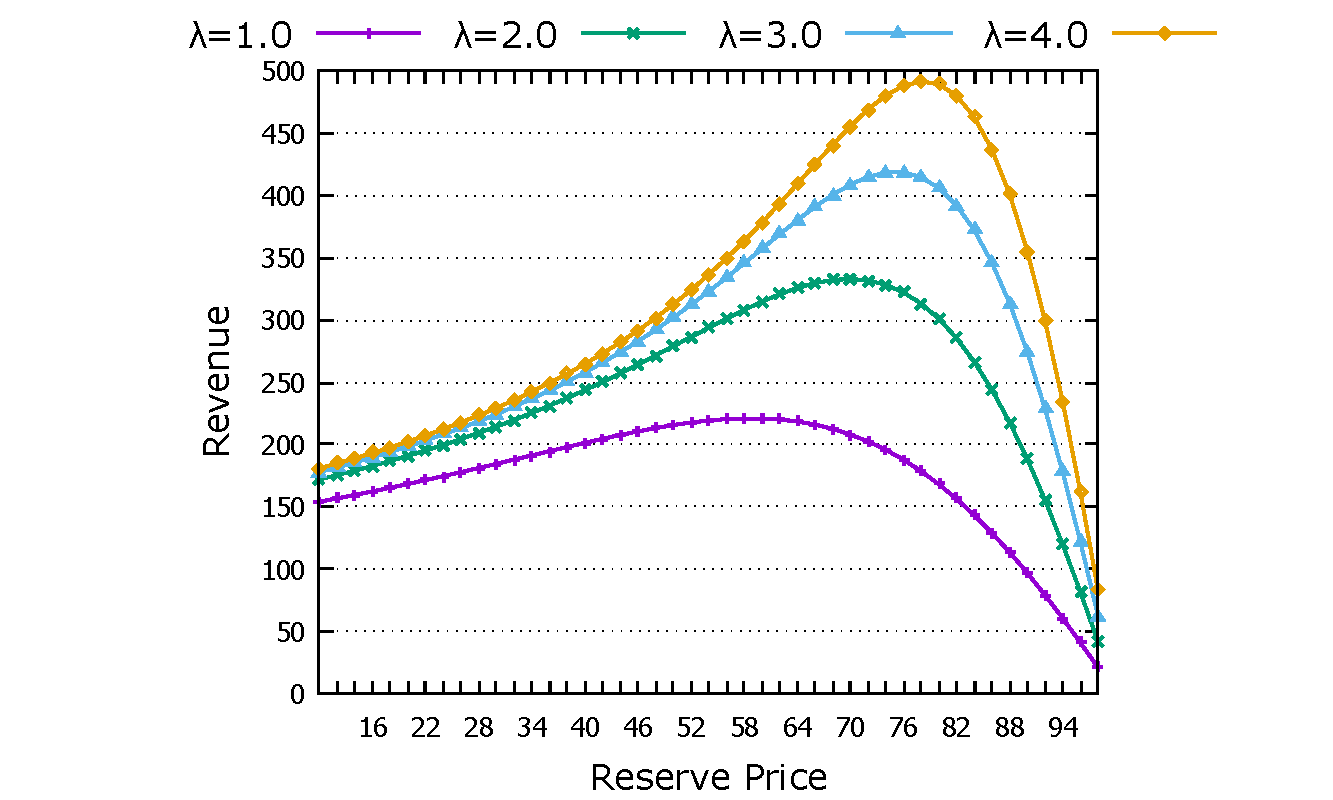
\includegraphics[width=0.4\textwidth]{chapter4/T=5vl=10vh=100.pdf}
	}
	\subfigure[$T=10,v_l=10,v_h=100$]{
		\label{fig:T=7vl=10vh=100}
		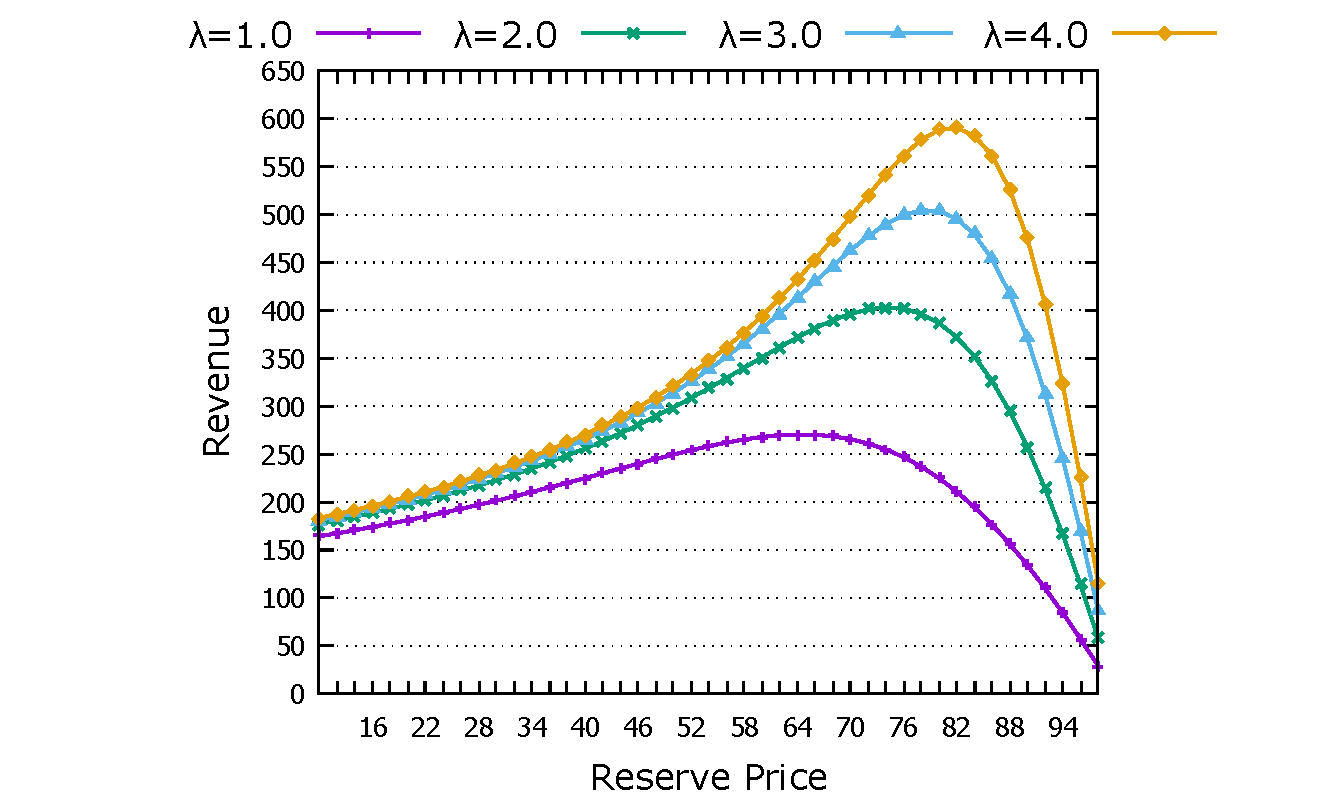
\includegraphics[width=0.4\textwidth]{chapter4/T=7vl=10vh=100.pdf}
	}
	\subfigure[$T=3,v_l=100,v_h=200$]{
		\label{fig:T=3vl=100vh=200}
		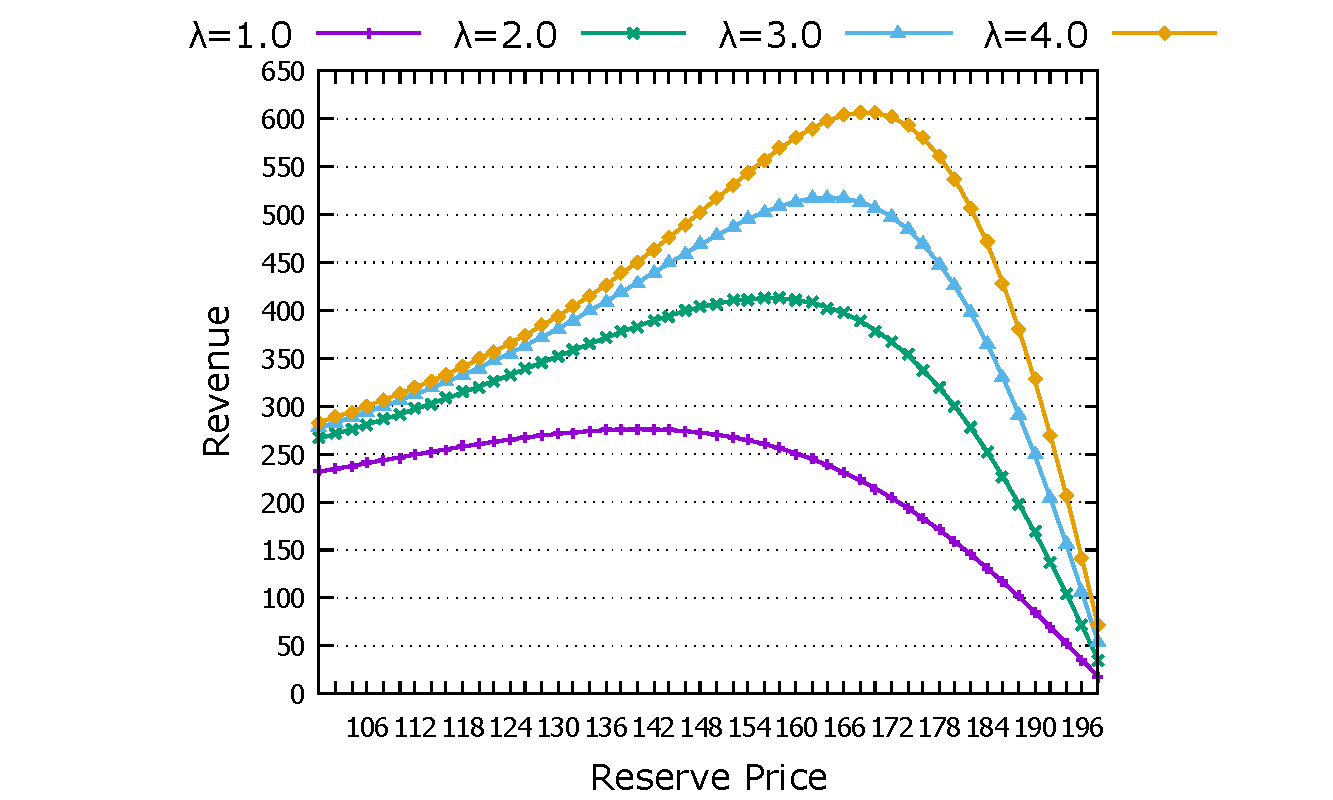
\includegraphics[width=0.4\textwidth]{chapter4/T=3vl=100vh=200.pdf}
	}
	\subfigure[$T=5,v_l=100,v_h=200$]{
		\label{fig:T=5vl=100vh=200}
		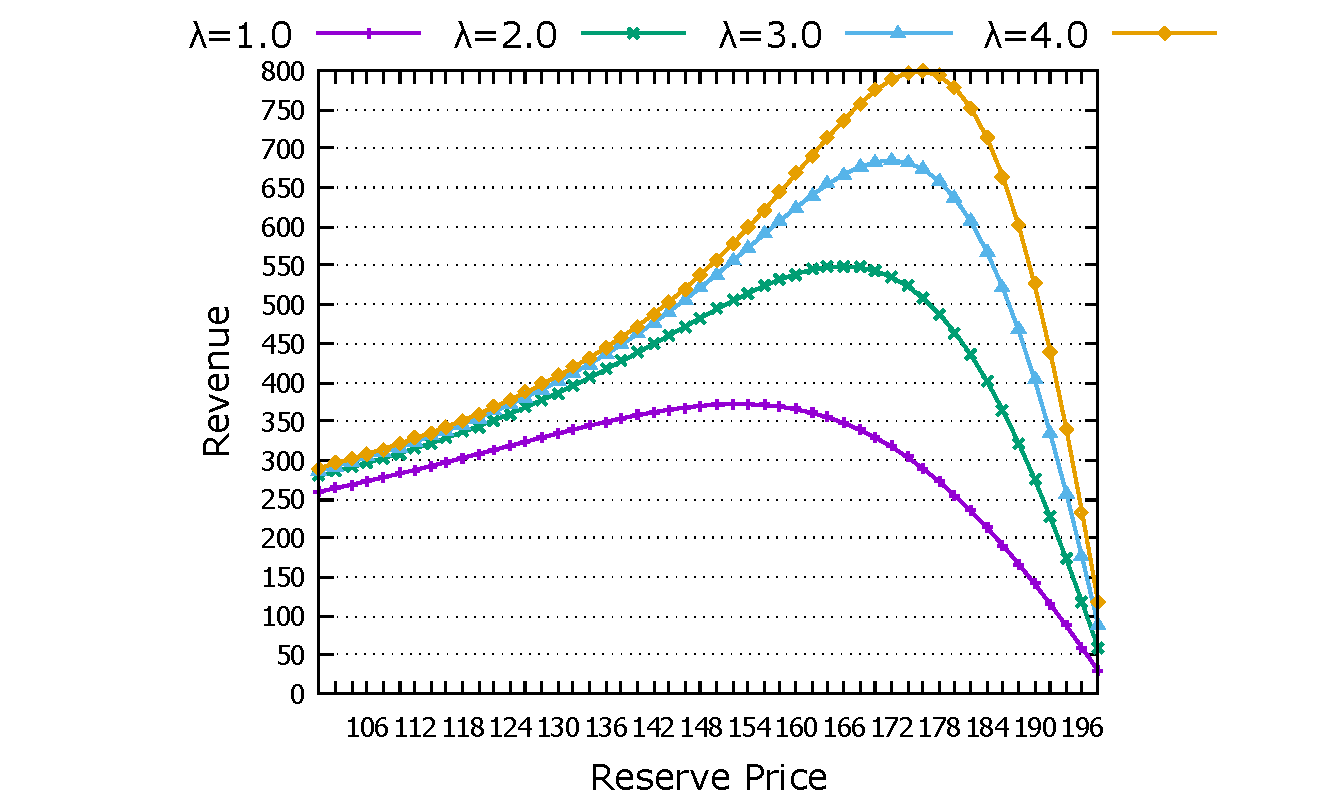
\includegraphics[width=0.4\textwidth]{chapter4/T=5vl=100vh=200.pdf}
	}
	\subfigure[$T=7,v_l=100,v_h=200$]{
		\label{fig:T=7vl=100vh=200}
		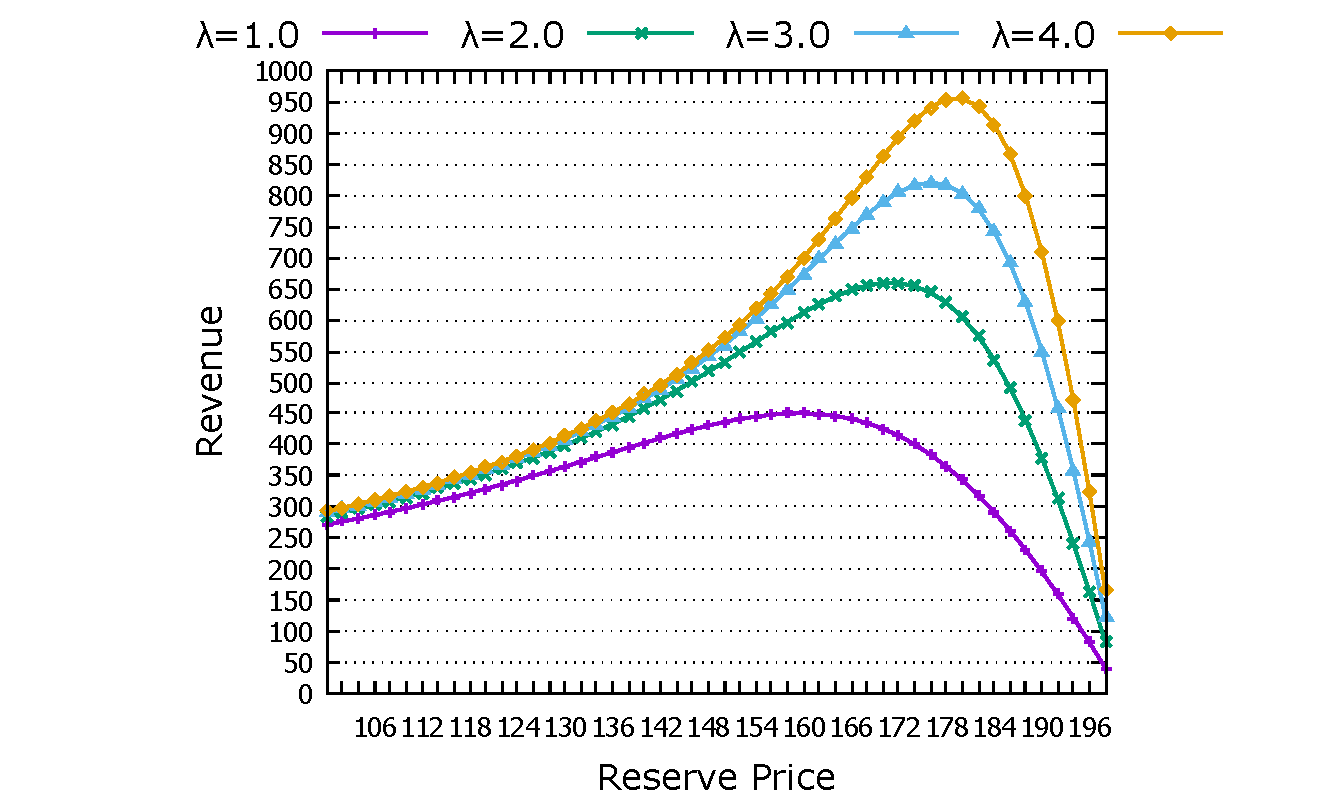
\includegraphics[width=0.4\textwidth]{chapter4/T=7vl=100vh=200.pdf}
	}
	\bicaption[fig:numercal result1]{在不同参数设置下的卖家平均收益与保留价的变化趋势}{在不同参数设置下的卖家平均收益与保留价的变化趋势}{Fig}{Relationship between revenue and reserve price under different parameter configurations}
\end{figure}

这里我们将拍卖时长$T$分别设置成$3,5,7$天,竞拍者到达率在[1.0,4.0]内变化。此外,我们还假设拍卖参与者的估价服从一个均匀分布,记为$v_i \thicksim U[v_l,v_h]$。我们选择$[10,100]$和$[100,200]$作为分布区间。接着,根据公式(\ref{eq:simplified online expected revenue})计算卖家的期望收益,计算结果绘制在图\ref{fig:numercal result1}中。




通过观察图\ref{fig:numercal result1}中,我们发现在每一个子图中所有曲线都呈现出相同的趋势,即卖家收益首先会随着保留价的增加而升高,随着保留价增加到最优保留价$r^*$而达到最大值,然后随着保留价的继续增加而下降。需要指出的是,我们这里的最优保留价$r^*$是根据命题\ref{proposition2}中的公式(\ref{eq:optimal reserve price})计算出来的。除此以外我们还观察到:1)那些有着更高到达率的曲线是能完全覆盖那些有着较低到达率的曲线;2)拍卖持续的时间越长,卖家期望收益越高;3)估价区间范围越大,卖家期望收益越高。

\subsection{成交价$E(v^{(2)})$的数值结果}

定义\ref{winning price definition}给出了第二价格在线拍卖中成交价$E(v^{(2)})$。类似于前面卖家期望收益的计算,在这里我们也将$E(v^{(2)})$的计算简化为:
\begin{equation}
\label{eq:simplified online expected winning price}
\begin{aligned}
E(v^{(2)}) = &\sum_{n=0}^{\infty}\frac{e^{-z}z^{n}}{n!} \int_{r}^{v_h} n(n-1)f(x)\\
&F^{(n-2)}(x)[1-F(x)]dx,
\end{aligned}
\end{equation}
其中$z=\lambda T(1-F(r))$,$T$是在线拍卖竞拍时长。

在$E(v^{(2)})$的结果展示中,我们的参数设置与前一小节相同。需要指出的是,这里的保留价也设置成之前计算出来的最优保留价,因为只有当保留价达到最优值时,$E(v^{(2)})$才会达到最大值。相关结果呈现在图\ref{fig:numercal result2}。

\begin{figure}[h]
	\centering
	\subfigure[$v_l=10,v_h=100$]{
		\label{fig:vl=10vh=100}
		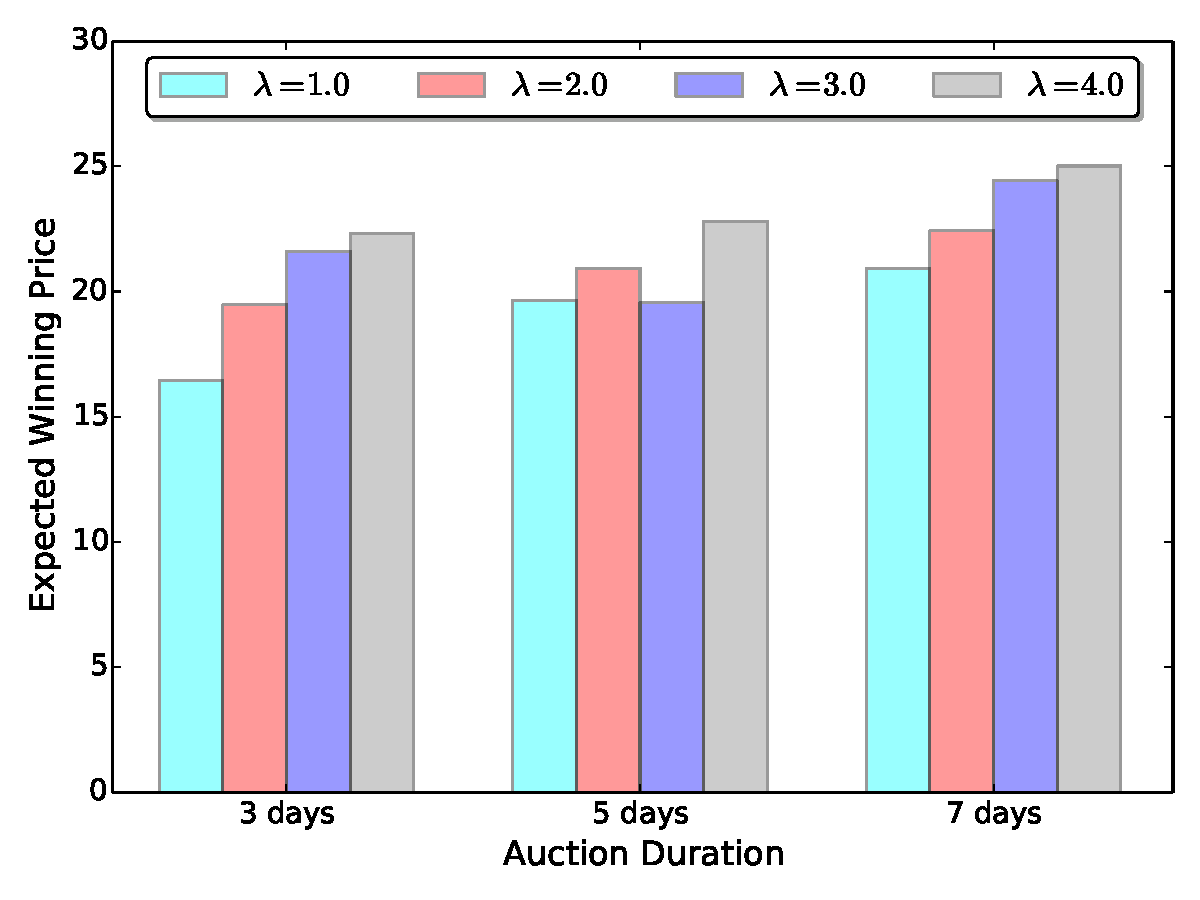
\includegraphics[width=0.55\textwidth]{chapter4/expected_price_vl=10vh=100.pdf}
	}
	\subfigure[$v_l=100,v_h=200$]{
		\label{fig:vl=100vh=200}
		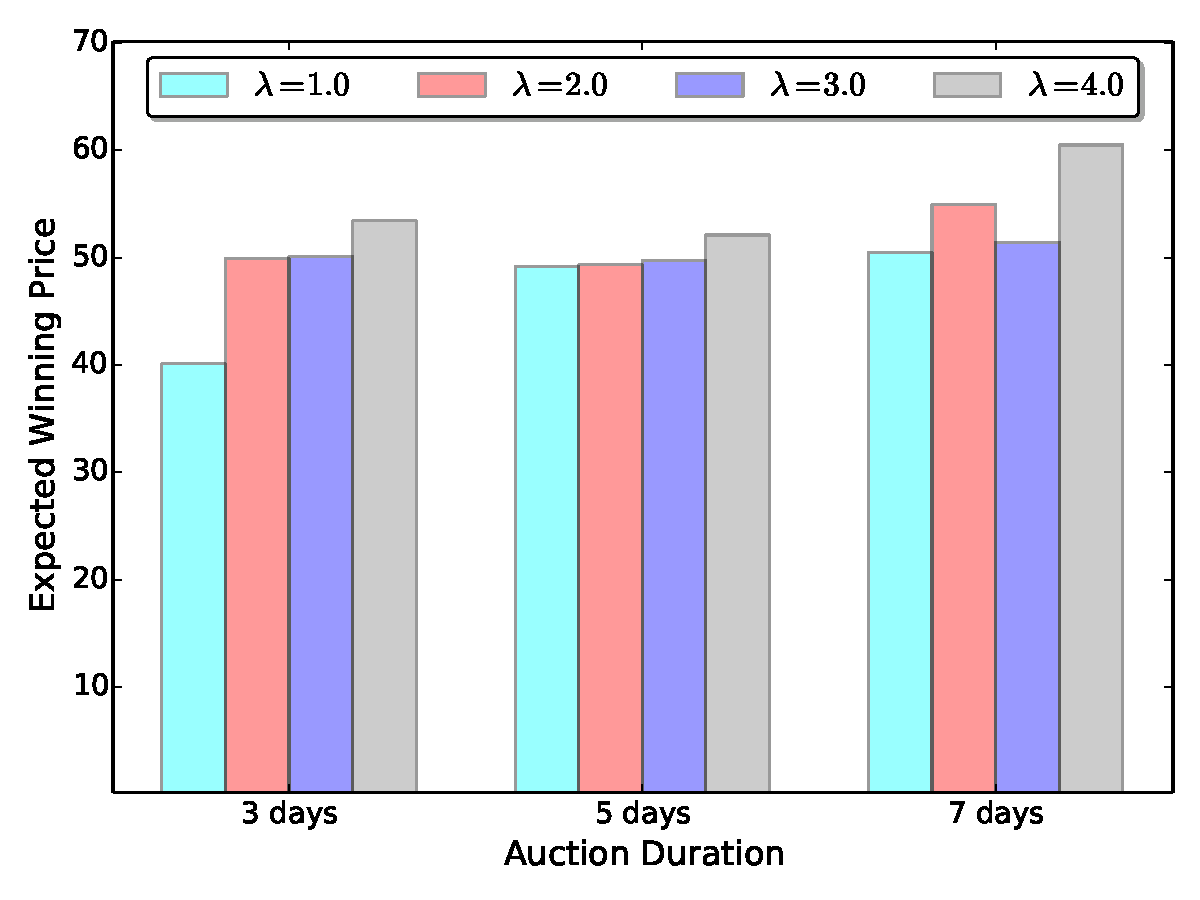
\includegraphics[width=0.55\textwidth]{chapter4/expected_price_vl=100vh=200.pdf}
	}
	\bicaption[fig:numercal result2]{在不同参数设置下的期望成交价$E(v^{(2)})$}{在不同参数设置下的期望成交价$E(v^{(2)})$}{Fig}{Numerical results of expected winning price $E(v^{(2)})$ under different parameter configurations}
\end{figure}

从图\ref{fig:numercal result2}中可以看出:1)拍卖持续时间越长,其拍品成交价就越高;2)较高的到达率会造成较高的期望成交价,这也意味着到达率可以一定程度上表示在线拍卖市场的竞争激烈程度;3)高估值的拍品最后的成交价都很高。

以上所有的数值结果与现有在线拍卖市场的经验调查是相符的,那么这意味着本文提出的模型是有能力模拟在线数据拍卖市场的。

\section{本章小结}

本小节提出了一个基于数据信息熵的在线数据拍卖模型。在叙述这个模型之前,我们分析了那些最影响现有传统商品在线拍卖的因素,比如拍卖机制、拍卖持续时长、拍卖参与人数以及保留价等等。在全面考虑了以上因素后,我们提出了基于数据信息熵的第$k$价格在线数据拍卖模型。在这个模型中,数据商品的数据信息熵被作为估价的参考。在这个模型的基础上,我们进一步分析了其最优保留价、期望成交价在不同出售数量下的变化趋势。此外,本文提出的一些命题和定义也在模型评估阶段进行了可视化的呈现。我们希望本文提出的模型和分析结果能给现有的在线数据拍卖市场提供些许启发,从而最大化拍卖参与者的总剩余,进一步繁荣整个数据市场。
%# -*- coding: utf-8-unix -*-
%%==================================================
%% conclusion.tex for SJTUThesis
%% Encoding: UTF-8
%%==================================================

\begin{summary}

这里是全文总结内容。

2015年2月28日,中央在北京召开全国精神文明建设工作表彰暨学雷锋志愿服务大会,公布全国文明城市(区)、文明村镇、文明单位名单。上海交通大学荣获全国文明单位称号。         

全国文明单位这一荣誉是对交大人始终高度重视文明文化工作的肯定,是对交大长期以来文明创建工作成绩的褒奖。在学校党委、文明委的领导下,交大坚持将文明创建工作纳入学校建设世界一流大学的工作中,全体师生医护员工群策群力、积极开拓,落实国家和上海市有关文明创建的各项要求,以改革创新、科学发展为主线,以质量提升为目标,聚焦文明创建工作出现的重点和难点,优化文明创建工作机制,传播学校良好形象,提升社会美誉度,显著增强学校软实力。2007至2012年间,上海交大连续三届荣获“上海市文明单位”称号,成为创建全国文明单位的新起点。         

上海交大自启动争创全国文明单位工作以来,凝魂聚气、改革创新,积极培育和践行社会主义核心价值观。坚持统筹兼顾、多措并举,将争创全国文明单位与学校各项中心工作紧密结合,着力构建学校文明创建新格局,不断提升师生医护员工文明素养,以“冲击世界一流大学汇聚强大精神动力”为指导思想,以“聚焦改革、多元推进、以评促建、丰富内涵、彰显特色”为工作原则,并由全体校领导群策领衔“党的建设深化、思想教育深入、办学成绩显著、大学文化丰富、校园环境优化、社会责任担当”六大板块共28项重点突破工作,全面展现近年来交大文明创建工作的全貌和成就。         

进入新阶段,学校将继续开拓文明创建工作新格局,不断深化工作理念和工作实践,创新工作载体、丰富活动内涵、凸显创建成效,积极服务于学校各项中心工作和改革发展的大局面,在上级党委、文明委的关心下,在学校党委的直接领导下,与时俱进、开拓创新,为深化内涵建设、加快建成世界一流大学、推动国家进步和社会发展而努力奋斗!       

上海交通大学医学院附属仁济医院也获得全国文明单位称号。      

\end{summary}

%%# -*- coding: utf-8-unix -*-
%%==================================================
%% chapter01.tex for SJTU Master Thesis
%%==================================================

%\bibliographystyle{sjtu2}%[此处用于每章都生产参考文献]
\chapter{这是什么}
\label{chap:intro}

这是上海交通大学(非官方)学位论文 \LaTeX 模板,当前版本是 \version 。

最早的一版学位模板是一位热心的物理系同学制作的。
那份模板参考了自动化所学位论文模板,使用了CASthesis.cls文档类,中文字符处理则采用当时最为流行的 \CJKLaTeX 方案。
我根据交大研究生院对学位论文的要求
\footnote{\url{http://www.gs.sjtu.edu.cn/policy/fileShow.ahtml?id=130}}
,结合少量个人审美喜好,完成了一份基本可用的交大 \LaTeX 学位论文模板。
但是,搭建一个 \CJKLaTeX 环境并不简单,单单在Linux下配置环境和添加中文字体,就足够让新手打退堂鼓。
在William Wang的建议下,我开始着手把模板向 \XeTeX 引擎移植。
他完成了最初的移植,多亏了他出色的工作,后续的改善工作也得以顺利进行。

随着我对 \LaTeX 系统认知增加,我又断断续续做了一些完善模板的工作,在原有硕士学位论文模板的基础上完成了交大学士和博士学位论文模板。

现在,交大学位论文模板SJTUTHesis代码在github
\footnote{\url{https://github.com/weijianwen/SJTUThesis}}
上维护。
你可以\href{https://github.com/weijianwen/SJTUThesis/issues}{在github上开issue}
、或者在\href{https://bbs.sjtu.edu.cn/bbsdoc?board=TeX_LaTeX}{水源LaTeX版}发帖来反映遇到的问题。

\section{使用模板}

\subsection{准备工作}
\label{sec:requirements}

要使用这个模板撰写学位论文,需要在\emph{TeX系统}、\emph{中英文字体}、\emph{TeX技能}上有所准备。

\begin{itemize}[noitemsep,topsep=0pt,parsep=0pt,partopsep=0pt]
	\item {\TeX}系统:所使用的{\TeX}系统要支持 \XeTeX 引擎,且带有ctex 2.x宏包,以2015年的\emph{完整}TeXLive、MacTeX发行版为佳。
	\item 中英文字体:操作系统中需要安装\footnote{在Windows、Mac OS X 以及 Linux 上安装额外的字体,可以参考\href{https://www.searchfreefonts.com/articles/how-to-install-fonts.htm}{“How to install fonts?”}。
}TeX Gyre Termes字体\footnote{\url{http://www.gust.org.pl/projects/e-foundry/tex-gyre/termes}}和四款Adobe中文字体
\footnote{请从合法渠道获得Adobe字体。}:AdobeSongStd、AdobeKaitiStd、AdobeHeitiStd、AdobeFangsongStd。
	\item TeX技能:尽管提供了对模板的必要说明,但这不是一份“ \LaTeX 入门文档”。在使用前请先通读其他入门文档。
	\item 针对Windows用户的额外需求:学位论文模本分别使用git和GNUMake进行版本控制和构建,建议从Cygwin\footnote{\url{http://cygwin.com}}安装这两个工具。
\end{itemize}

\subsection{模板选项}
\label{sec:thesisoption}

sjtuthesis提供了一些常用选项,在thesis.tex在导入sjtuthesis模板类时,可以组合使用。
这些选项包括:

\begin{itemize}[noitemsep,topsep=0pt,parsep=0pt,partopsep=0pt]
\item 学位类型:bachelor(学位)、master(硕士)、doctor(博士),是必选项。
\item 中国字体:adobefonts(Adobe中文字体)、winfonts(使用Windows下的中文字体,该选项未在Linux/Mac下测试)。
\item 正文字号:cs4size(小四)、c5size(五号)。
\item 盲审选项:使用review选项后,论文作者、学号、导师姓名、致谢、发表论文和参与项目将被隐去。
\end{itemize}

\subsection{编译模板}
\label{sec:process}

模板默认使用GNUMake构建,GNUMake将调用latemk工具自动完成模板多轮编译:

\begin{lstlisting}[basicstyle=\small\ttfamily, caption={编译模板}, numbers=none]
make clean thesis.pdf
\end{lstlisting}

若需要生成包含“原创性声明扫描件”的学位论文文档,请将扫描件保存为statement.pdf,然后调用make生成submit.pdf。

\begin{lstlisting}[basicstyle=\small\ttfamily, caption={生成用于提交的学位论文}, numbers=none]
make clean submit.pdf
\end{lstlisting}

编译失败时,可以尝试手动逐次编译,定位故障。

\begin{lstlisting}[basicstyle=\small\ttfamily, caption={手动逐次编译}, numbers=none]
xelatex -no-pdf thesis
biber --debug thesis
xelatex thesis
xelatex thesis
\end{lstlisting}

\subsection{模板文件布局}
\label{sec:layout}

\begin{lstlisting}[basicstyle=\small\ttfamily,caption={模板文件布局},label=layout,float,numbers=none]
├── LICENSE
├── Makefile
├── README.md
├── bib
│   ├── chap1.bib
│   └── chap2.bib
├── bst
│   └── GBT7714-2005NLang.bst
├── figure
│   ├── chap2
│   │   ├── sjtulogo.eps
│   │   ├── sjtulogo.jpg
│   │   ├── sjtulogo.pdf
│   │   └── sjtulogo.png
│   └── sjtubanner.png
├── sjtuthesis.cfg
├── sjtuthesis.cls
├── statement.pdf
├── submit.pdf
├── tex
│   ├── abstract.tex
│   ├── ack.tex
│   ├── app_cjk.tex
│   ├── app_eq.tex
│   ├── app_log.tex
│   ├── chapter01.tex
│   ├── chapter02.tex
│   ├── chapter03.tex
│   ├── conclusion.tex
│   ├── id.tex
│   ├── patents.tex
│   ├── projects.tex
│   ├── pub.tex
│   └── symbol.tex
└── thesis.tex
\end{lstlisting}

本节介绍学位论文模板中木要文件和目录的功能。

\subsubsection{格式控制文件}
\label{sec:format}

格式控制文件控制着论文的表现形式,包括以下几个文件:
sjtuthesis.cfg, sjtuthesis.cls和GBT7714-2005NLang.bst。
其中,“cfg”和“cls”控制论文主体格式,“bst”控制参考文献条目的格式,

\subsubsection{主控文件thesis.tex}
\label{sec:thesistex}

主控文件thesis.tex的作用就是将你分散在多个文件中的内容“整合”成一篇完整的论文。
使用这个模板撰写学位论文时,你的学位论文内容和素材会被“拆散”到各个文件中:
譬如各章正文、各个附录、各章参考文献等等。
在thesis.tex中通过“include”命令将论文的各个部分包含进来,从而形成一篇结构完成的论文。
对模板定制时引入的宏包,建议放在导言区。

\subsubsection{各章源文件tex}
\label{sec:thesisbody}

这一部分是论文的主体,是以“章”为单位划分的,包括:

\begin{itemize}[noitemsep,topsep=0pt,parsep=0pt,partopsep=0pt]
	\item 中英文摘要(abstract.tex)。前言(frontmatter)的其他部分,中英文封面、原创性声明、授权信息在sjtuthesis.cls中定义,不单独分离为tex文件。
不单独弄成文件。
	\item 正文(mainmatter)——学位论文正文的各章内容,源文件是chapter\emph{xxx}.tex。
	\item 附录(app\emph{xx}.tex)、致谢(thuanks.tex)、攻读学位论文期间发表的学术论文目录(pub.tex)、个人简历(resume.tex)组成正文后的部分(backmatter)。
参考文献列表由bibtex插入,不作为一个单独的文件。
\end{itemize}

\subsubsection{图片文件夹figure}
\label{sec:fig}

figure文件夹放置了需要插入文档中的图片文件(支持PNG/JPG/PDF/EPS格式的图片),可以在按照章节划分子目录。
模板文件中使用\verb|\graphicspath|命令定义了图片存储的顶层目录,在插入图片时,顶层目录名“figure”可省略。

\subsubsection{参考文献数据库bib}
\label{sec:bib}

目前参考文件数据库目录只存放一个参考文件数据库thesis.bib。
关于参考文献引用,可参考第\ref{chap:example}章中的例子。


%%# -*- coding: utf-8-unix -*-
%%==================================================
%% chapter02.tex for SJTU Master Thesis
%% based on CASthesis
%% modified by wei.jianwen@gmail.com
%% Encoding: UTF-8
%%==================================================

\chapter{ \LaTeX 排版例子}
\label{chap:example}

\section{列表环境}
\label{sec:list}

\subsection{无序列表}
\label{sec:unorderlist}

以下是一个无序列表的例子,列表的每个条目单独分段。

\begin{itemize}
  \item 这是一个无序列表。
  \item 这是一个无序列表。
  \item 这是一个无序列表。
\end{itemize}

使用\verb+itemize*+环境可以创建行内无序列表。
\begin{itemize*}
  \item 这是一个无序列表。
  \item 这是一个无序列表。
  \item 这是一个无序列表。
\end{itemize*}
行内无序列表条目不单独分段,所有内容直接插入在原文的段落中。

\subsection{有序列表}
\label{sec:orderlist}

使用环境\verb+enumerate+和\verb+enumerate*+创建有序列表,
使用方法无序列表类似。

\begin{enumerate}
  \item 这是一个有序列表。
  \item 这是一个有序列表。
  \item 这是一个有序列表。
\end{enumerate}

使用\verb+enumerate*+环境可以创建行内有序列表。
\begin{enumerate*}
  \item 这是一个默认有序列表。
  \item 这是一个默认有序列表。
  \item 这是一个默认有序列表。
\end{enumerate*}
行内有序列表条目不单独分段,所有内容直接插入在原文的段落中。

\subsection{描述型列表}

使用环境\verb+description+可创建带有主题词的列表,条目语法是\verb+\item[主题] 内容+。
\begin{description}
    \item[主题一] 详细内容
    \item[主题二] 详细内容
    \item[主题三] 详细内容 \ldots
\end{description}

\subsection{自定义列表样式}

可以使用\verb+label+参数控制列表的样式,
详细可以参考WikiBooks\footnote{\url{https://en.wikibooks.org/wiki/LaTeX/List_Structures\#Customizing_lists}}。
比如一个自定义样式的行内有序列表
\begin{enumerate*}[label=\itshape\alph*)\upshape]
  \item 这是一个自定义样式有序列表。
  \item 这是一个自定义样式有序列表。
  \item 这是一个自定义样式有序列表。
\end{enumerate*}

\section{数学排版}
\label{sec:matheq}

\subsection{公式排版}
\label{sec:eqformat}

这里有举一个长公式排版的例子,来自\href{http://www.tex.ac.uk/tex-archive/info/math/voss/mathmode/Mathmode.pdf}{《Math mode》}:

\begin {multline}
  \frac {1}{2}\Delta (f_{ij}f^{ij})=
  2\left (\sum _{i<j}\chi _{ij}(\sigma _{i}-
    \sigma _{j}) ^{2}+ f^{ij}\nabla _{j}\nabla _{i}(\Delta f)+\right .\\
  \left .+\nabla _{k}f_{ij}\nabla ^{k}f^{ij}+
    f^{ij}f^{k}\left [2\nabla _{i}R_{jk}-
      \nabla _{k}R_{ij}\right ]\vphantom {\sum _{i<j}}\right )
\end{multline}

\subsection{SI单位}

使用\verb+siunitx+宏包可以方便地输入SI单位制单位,例如\verb+\SI{5}{\um}+可以得到\SI{5}{\um}。

\subsubsection{一个四级标题}
\label{sec:depth4}

这是全文唯一的一个四级标题。在这部分中将演示了mathtools宏包中可伸长符号(箭头、等号的例子)的例子。

\begin{displaymath}
    A \xleftarrow[n=0]{} B \xrightarrow[LongLongLongLong]{n>0} C 
\end{displaymath}

\begin{eqnarray}
  f(x) & \xleftrightarrow[]{A=B}  & B \\
  & \xleftharpoondown[below]{above} & B \nonumber \\
  & \xLeftrightarrow[below]{above} & B
\end{eqnarray}

又如:

\begin{align}
  \label{eq:none}
  & I(X_3;X_4)-I(X_3;X_4\mid{}X_1)-I(X_3;X_4\mid{}X_2) \nonumber \\
  = & [I(X_3;X_4)-I(X_3;X_4\mid{}X_1)]-I(X_3;X_4\mid{}\tilde{X}_2) \\
  = & I(X_1;X_3;X_4)-I(X_3;X_4\mid{}\tilde{X}_2)
\end{align}

\subsection{定理环境}

模板中定义了丰富的定理环境
algo(算法),thm(定理),lem(引理),prop(命题),cor(推论),defn(定义),conj(猜想),exmp(例),rem(注),case(情形),
bthm(断言定理),blem(断言引理),bprop(断言命题),bcor(断言推论)。
amsmath还提供了一个proof(证明)的环境。
这里举一个“定理”和“证明”的例子。
\begin{thm}[留数定理]
\label{thm:res}
  假设$U$是复平面上的一个单连通开子集,$a_1,\ldots,a_n$是复平面上有限个点,$f$是定义在$U\backslash \{a_1,\ldots,a_n\}$上的全纯函数,
  如果$\gamma$是一条把$a_1,\ldots,a_n$包围起来的可求长曲线,但不经过任何一个$a_k$,并且其起点与终点重合,那么:

  \begin{equation}
    \label{eq:res}
    \ointop_{\gamma}f(z)\,\mathrm{d}z = 2\uppi\mathbf{i}\sum^n_{k=1}\mathrm{I}(\gamma,a_k)\mathrm{Res}(f,a_k)
  \end{equation}

  如果$\gamma$是若尔当曲线,那么$\mathrm{I}(\gamma, a_k)=1$,因此:

  \begin{equation}
    \label{eq:resthm}
    \ointop_{\gamma}f(z)\,\mathrm{d}z = 2\uppi\mathbf{i}\sum^n_{k=1}\mathrm{Res}(f,a_k)
  \end{equation}

      % \oint_\gamma f(z)\, dz = 2\pi i \sum_{k=1}^n \mathrm{Res}(f, a_k ). 

  在这里,$\mathrm{Res}(f, a_k)$表示$f$在点$a_k$的留数,$\mathrm{I}(\gamma,a_k)$表示$\gamma$关于点$a_k$的卷绕数。
  卷绕数是一个整数,它描述了曲线$\gamma$绕过点$a_k$的次数。如果$\gamma$依逆时针方向绕着$a_k$移动,卷绕数就是一个正数,
  如果$\gamma$根本不绕过$a_k$,卷绕数就是零。

  定理\ref{thm:res}的证明。
  
  \begin{proof}
    首先,由……

    其次,……

    所以……
  \end{proof}
\end{thm}

上面的公式例子中,有一些细节希望大家注意。微分号d应该使用“直立体”也就是用mathrm包围起来。
并且,微分号和被积函数之间应该有一段小间隔,可以插入\verb+\,+得到。
斜体的$d$通常只作为一般变量。
i,j作为虚数单位时,也应该使用“直立体”为了明显,还加上了粗体,例如\verb+\mathbf{i}+。斜体$i,j$通常用作表示“序号”。
其他字母在表示常量时,也推荐使用“直立体”譬如,圆周率$\uppi$(需要upgreek宏包),自然对数的底$\mathrm{e}$。
不过,我个人觉得斜体的$e$和$\pi$很潇洒,在不至于引起混淆的情况下,我也用这两个字母的斜体表示对应的常量。


\section{向文档中插入图像}
\label{sec:insertimage}

\subsection{支持的图片格式}
\label{sec:imageformat}

\XeTeX 可以很方便地插入PDF、PNG、JPG格式的图片。

插入PNG/JPG的例子如\ref{fig:SRR}所示。
这两个水平并列放置的图共享一个“图标题”(table caption),没有各自的小标题。

\begin{figure}[!htp]
  \centering
  
\includegraphics[width=0.3\textwidth]{example/sjtulogo.png}
  \hspace{1cm}
  
\includegraphics[width=0.3\textwidth]{example/sjtulogo.jpg}
  \bicaption[fig:SRR]{这里将出现在插图索引中}{中文题图}{Fig}{English caption}
\end{figure}

% 这里还有插入eps图像和pdf图像的例子,如图\ref{fig:epspdf:a}和图\ref{fig:epspdf:b}。这里将EPS和PDF图片作为子图插入,每个子图有自己的小标题。并列子图的功能是使用subfigure宏包提供的。
% 
% \begin{figure}
%   \centering
%   \subfigure[EPS Figure]{
%     \label{fig:epspdf:a} %% label for first subfigure
%     
\includegraphics[width=0.3\textwidth]{example/sjtulogo.eps}}
%   \hspace{1in}
%   \subfigure[PDF Figure]{
%     \label{fig:epspdf:b} %% label for second subfigure
%     
\includegraphics[width=0.3\textwidth]{example/sjtulogo.pdf}}
%   \bicaption[fig:pdfeps]{插入eps图像和pdf图像}{插入eps和pdf的例子}{Fig}{An EPS and PDF demo}
% \end{figure}

更多关于 \LaTeX 插图的例子可以参考\href{http://www.cs.duke.edu/junhu/Graphics3.pdf}{《\LaTeX 插图指南》}。

\subsection{长标题的换行}
\label{sec:longcaption}

图\ref{fig:longcaptionbad}和图\ref{fig:longcaptiongood}都有比较长图标题,通过对比发现,图\ref{fig:longcaptiongood}的换行效果更好一些。
其中使用了minipage环境来限制整个浮动体的宽度。

\begin{figure}[!htp]
 \centering
 
\includegraphics[width=4cm]{example/sjtulogo.pdf}
 \bicaption[fig:longcaptionbad]{这里将出现在插图索引}{海交通大学是我国历史最悠久的高等学府之一,是教育部直属、教育部与上海市共建的全国重点大学.}{Fig}{Where there is a will, there is a way.}
\end{figure}

\begin{figure}[!htbp]
  \centering
  \begin{minipage}[b]{0.6\textwidth}
    \captionstyle{\centering}
    \centering
    
\includegraphics[width=4cm]{example/sjtulogo.pdf}
    \bicaption[fig:longcaptiongood]{这里将出现在插图索引}{海交通大学是我国历史最悠久的高等学府之一,是教育部直属、教育部与上海市共建的全国重点大学.}{Fig}{Where there is a will, there is a way.}
  \end{minipage}     
\end{figure}

\subsection{绘制流程图}

图\ref{fig:flow_chart}是一张流程图示意。使用tikz环境,搭配四种预定义节点(\verb+startstop+、\verb+process+、\verb+decision+和\verb+io+),可以容易地绘制出流程图。
\begin{figure}[!htp]
    \centering
    \resizebox{6cm}{!}{\begin{tikzpicture}[node distance=2cm]
    \node (pic) [startstop] {待测图片};
    \node (bg) [io, below of=pic] {读取背景};
    \node (pair) [process, below of=bg] {匹配特征点对};
    \node (threshold) [decision, below of=pair, yshift=-0.5cm] {多于阈值};
    \node (clear) [decision, right of=threshold, xshift=3cm] {清晰?};
    \node (capture) [process, right of=pair, xshift=3cm, yshift=0.5cm] {重采};
    \node (matrix_p) [process, below of=threshold, yshift=-0.8cm] {透视变换矩阵};
    \node (matrix_a) [process, right of=matrix_p, xshift=3cm] {仿射变换矩阵};
    \node (reg) [process, below of=matrix_p] {图像修正};
    \node (return) [startstop, below of=reg] {配准结果};
     
    %连接具体形状
    \draw [arrow](pic) -- (bg);
    \draw [arrow](bg) -- (pair);
    \draw [arrow](pair) -- (threshold);

    \draw [arrow](threshold) -- node[anchor=south] {否} (clear);

    \draw [arrow](clear) -- node[anchor=west] {否} (capture);
    \draw [arrow](capture) |- (pic);
    \draw [arrow](clear) -- node[anchor=west] {是} (matrix_a);
    \draw [arrow](matrix_a) |- (reg);

    \draw [arrow](threshold) -- node[anchor=east] {是} (matrix_p);
    \draw [arrow](matrix_p) -- (reg);
    \draw [arrow](reg) -- (return);
\end{tikzpicture}
}
    \bicaption[fig:flow_chart]{绘制流程图效果}{流程图}{Fig}{Flow chart}
\end{figure}
  
\clearpage

\section{表格}
\label{sec:tab}

这一节给出的是一些表格的例子,如表\ref{tab:firstone}所示。

\begin{table}[!hpb]
  \centering
  \bicaption[tab:firstone]{指向一个表格的表目录索引}{一个颇为标准的三线表格\footnotemark[1]}{Table}{A Table}
  \begin{tabular}{@{}llr@{}} \toprule
    \multicolumn{2}{c}{Item} \\ \cmidrule(r){1-2}
    Animal & Description & Price (\$)\\ \midrule
    Gnat & per gram & 13.65 \\
    & each & 0.01 \\
    Gnu & stuffed & 92.50 \\
    Emu & stuffed & 33.33 \\
    Armadillo & frozen & 8.99 \\ \bottomrule
  \end{tabular}
\end{table}
\footnotetext[1]{这个例子来自\href{http://www.ctan.org/tex-archive/macros/latex/contrib/booktabs/booktabs.pdf}{《Publication quality tables in LATEX》}(booktabs宏包的文档)。这也是一个在表格中使用脚注的例子,请留意与threeparttable实现的效果有何不同。}

下面一个是一个更复杂的表格,用threeparttable实现带有脚注的表格,如表\ref{tab:footnote}。

\begin{table}[!htpb]
  \bicaption[tab:footnote]{出现在表目录的标题}{一个带有脚注的表格的例子}{Table}{A Table with footnotes}
  \centering
  \begin{threeparttable}[b]
     \begin{tabular}{ccd{4}cccc}
      \toprule
      \multirow{2}{6mm}{total}&\multicolumn{2}{c}{20\tnote{1}} & \multicolumn{2}{c}{40} &  \multicolumn{2}{c}{60}\\
      \cmidrule(lr){2-3}\cmidrule(lr){4-5}\cmidrule(lr){6-7}
      &www & k & www & k & www & k \\
      \midrule
      &$\underset{(2.12)}{4.22}$ & 120.0140\tnote{2} & 333.15 & 0.0411 & 444.99 & 0.1387 \\
      &168.6123 & 10.86 & 255.37 & 0.0353 & 376.14 & 0.1058 \\
      &6.761    & 0.007 & 235.37 & 0.0267 & 348.66 & 0.1010 \\
      \bottomrule
    \end{tabular}
    \begin{tablenotes}
    \item [1] the first note.% or \item [a]
    \item [2] the second note.% or \item [b]
    \end{tablenotes}
  \end{threeparttable}
\end{table}

\section{参考文献管理}

 \LaTeX 具有将参考文献内容和表现形式分开管理的能力,涉及三个要素:参考文献数据库、参考文献引用格式、在正文中引用参考文献。
这样的流程需要多次编译:

\begin{enumerate}[noitemsep,topsep=0pt,parsep=0pt,partopsep=0pt]
	\item 用户将论文中需要引用的参考文献条目,录入纯文本数据库文件(bib文件)。
	\item 调用xelatex对论文模板做第一次编译,扫描文中引用的参考文献,生成参考文献入口文件(aux)文件。
	\item 调用bibtex,以参考文献格式和入口文件为输入,生成格式化以后的参考文献条目文件(bib)。
	\item 再次调用xelatex编译模板,将格式化以后的参考文献条目插入正文。
\end{enumerate}

参考文献数据库(thesis.bib)的条目,可以从Google Scholar搜索引擎\footnote{\url{https://scholar.google.com}}、CiteSeerX搜索引擎\footnote{\url{http://citeseerx.ist.psu.edu}}中查找,文献管理软件Papers\footnote{\url{http://papersapp.com}}、Mendeley\footnote{\url{http://www.mendeley.com}}、JabRef\footnote{\url{http://jabref.sourceforge.net}}也能够输出条目信息。

下面是在Google Scholar上搜索到的一条文献信息,格式是纯文本:

\begin{lstlisting}[caption={从Google Scholar找到的参考文献条目}, label=googlescholar, escapeinside="", numbers=none]
    @phdthesis{"白2008信用风险传染模型和信用衍生品的定价",
      title={"信用风险传染模型和信用衍生品的定价"},
      author={"白云芬"},
      year={2008},
      school={"上海交通大学"}
    } 
\end{lstlisting}

推荐修改后在bib文件中的内容为:

\begin{lstlisting}[caption={修改后的参考文献条目}, label=itemok, escapeinside="", numbers=none]
  @phdthesis{bai2008,
    title={"信用风险传染模型和信用衍生品的定价"},
    author={"白云芬"},
    date={2008},
    address={"上海"},
    school={"上海交通大学"}
  } 
\end{lstlisting}

按照教务处的要求,参考文献外观应符合国标GBT7714的要求\footnote{\url{http://www.cces.net.cn/guild/sites/tmxb/Files/19798_2.pdf}}。
在模板中,表现形式的控制逻辑通过bibla­tex-gb7714-2015包实现\footnote{\url{https://www.ctan.org/pkg/biblatex-gb7714-2015}},基于{Bib\LaTeX}管理文献。在目前的多数TeX发行版中,可能都没有默认包含biblatex-gb7714-2015,需要手动安装。

正文中引用参考文献时,用\verb+\cite{key1,key2,key3...}+可以产生“上标引用的参考文献”,
如\cite{Meta_CN,chen2007act,DPMG}。
使用\verb+\citen{key1,key2,key3...}+则可以产生水平引用的参考文献,例如\citen{JohnD,zhubajie,IEEE-1363}。
请看下面的例子,将会穿插使用水平的和上标的参考文献:关于书的\citen{Meta_CN,JohnD,IEEE-1363},关于期刊的\cite{chen2007act,chen2007ewi},
会议论文\citen{DPMG,kocher99,cnproceed},
硕士学位论文\citen{zhubajie,metamori2004},博士学位论文\cite{shaheshang,FistSystem01,bai2008},标准文件\citen{IEEE-1363},技术报告\cite{NPB2},电子文献\citen{xiaoyu2001, CHRISTINE1998},用户手册\citen{RManual}。

总结一些注意事项:
\begin{itemize}
\item 参考文献只有在正文中被引用了,才会在最后的参考文献列表中出现;
\item 参考文献“数据库文件”bib是纯文本文件,请使用UTF-8编码,不要使用GBK编码;
\item 参考文献条目中默认通过date域输入时间。兼容使用year域时会产生编译warning,可忽略。
\end{itemize}

\section{用listings插入源代码}

原先ctexbook文档类和listings宏包配合使用时,代码在换页时会出现莫名其妙的错误,后来经高人指点,顺利解决了。
感兴趣的话,可以看看\href{http://bbs.ctex.org/viewthread.php?tid=53451}{这里}。
这里给使用listings宏包插入源代码的例子,这里是一段C代码。
另外,listings宏包真可谓博大精深,可以实现各种复杂、漂亮的效果,想要进一步学习的同学,可以参考
\href{http://mirror.ctan.org/macros/latex/contrib/listings/listings.pdf}{listings宏包手册}。

\begin{lstlisting}[language={C}, caption={一段C源代码}]
#include <stdio.h>
#include <unistd.h>
#include <sys/types.h>
#include <sys/wait.h>

int main() {
  pid_t pid;

  switch ((pid = fork())) {
  case -1:
    printf("fork failed\n");
    break;
  case 0:
    /* child calls exec */
    execl("/bin/ls", "ls", "-l", (char*)0);
    printf("execl failed\n");
    break;
  default:
    /* parent uses wait to suspend execution until child finishes */
    wait((int*)0);
    printf("is completed\n");
    break;
  }

  return 0;
}
\end{lstlisting}

\section{用algorithm和algorithmicx宏包插入算法描述}

algorithmicx 比 algorithmic 增加了一些命令。
示例如算法\ref{algo:sum_100}和算法\ref{algo:merge_sort},
后者的代码来自\href{http://hustsxh.is-programmer.com/posts/38801.html}{xhSong的博客}。
algorithmicx的详细使用方法见\href{http://mirror.hust.edu.cn/CTAN/macros/latex/contrib/algorithmicx/algorithmicx.pdf}{官方README}。
使用算法宏包时,算法出现的位置很多时候不按照tex文件里的书写顺序, 
需要强制定位时可以使用\verb+\begin{algorithm}[H]+
\footnote{http://tex.stackexchange.com/questions/165021/fixing-the-location-of-the-appearance-in-algorithmicx-environment}

这是写在算法\ref{algo:sum_100}前面的一段话,在生成的文件里它会出现在算法\ref{algo:sum_100}前面。

\begin{algorithm}
% \begin{algorithm}[H] % 强制定位
\caption{求100以内的整数和}
\label{algo:sum_100}
\begin{algorithmic}[1] %每行显示行号
\Ensure 100以内的整数和 % 输出
\State $sum \gets 0$
\For{$i = 0 \to 100$}
    \State $sum \gets sum + i$
  \EndFor
\end{algorithmic}
\end{algorithm}

这是写在两个算法中间的一段话,当算法\ref{algo:sum_100}不使用\verb+\begin{algorithm}[H]+时它也会出现在算法\ref{algo:sum_100}前面。

对于很长的算法,单一的算法块\verb+\begin{algorithm}...\end{algorithm}+是不能自动跨页的
\footnote{http://tex.stackexchange.com/questions/70733/latex-algorithm-not-display-under-correct-section},
会出现的情况有:

\begin{itemize}
  \item 该页放不下当前的算法,留下大片空白,算法在下一页显示
  \item 单一页面放不下当前的算法,显示时超过页码的位置直到超出整个页面范围
\end{itemize}

解决方法有:

\begin{itemize}
  \item (推荐)使用\verb+algstore{algname}+和\verb+algrestore{algname}+来讲算法分为两个部分\footnote{http://tex.stackexchange.com/questions/29816/algorithm-over-2-pages},如算法\ref{algo:merge_sort}。
  \item 人工拆分算法为多个小的部分。
\end{itemize}

\begin{algorithm}
% \begin{algorithm}[H] % 强制定位
\caption{用归并排序求逆序数}
\label{algo:merge_sort}
\begin{algorithmic}[1] %每行显示行号
\Require $Array$数组,$n$数组大小 % 输入
\Ensure 逆序数 % 输出
\Function {MergerSort}{$Array, left, right$}
  \State $result \gets 0$
  \If {$left < right$}
    \State $middle \gets (left + right) / 2$
    \State $result \gets result +$ \Call{MergerSort}{$Array, left, middle$}
    \State $result \gets result +$ \Call{MergerSort}{$Array, middle, right$}
    \State $result \gets result +$ \Call{Merger}{$Array,left,middle,right$}
  \EndIf
  \State \Return{$result$}
\EndFunction
\State %空一行
\Function{Merger}{$Array, left, middle, right$}
  \State $i\gets left$
  \State $j\gets middle$
  \State $k\gets 0$
  \State $result \gets 0$
  \While{$i<middle$ \textbf{and} $j<right$}
    \If{$Array[i]<Array[j]$}
      \State $B[k++]\gets Array[i++]$
    \Else
      \State $B[k++] \gets Array[j++]$
      \State $result \gets result + (middle - i)$
    \EndIf
  \EndWhile
  \algstore{MergeSort}
\end{algorithmic}
\end{algorithm}

\begin{algorithm}
\begin{algorithmic}[1]
  \algrestore{MergeSort}
  \While{$i<middle$}
    \State $B[k++] \gets Array[i++]$
  \EndWhile
  \While{$j<right$}
    \State $B[k++] \gets Array[j++]$
  \EndWhile
  \For{$i = 0 \to k-1$}
    \State $Array[left + i] \gets B[i]$
  \EndFor
  \State \Return{$result$}
\EndFunction
\end{algorithmic}
\end{algorithm}

这是写在算法\ref{algo:merge_sort}后面的一段话,
但是当算法\ref{algo:merge_sort}不使用\verb+\begin{algorithm}[H]+时它会出现在算法\ref{algo:merge_sort}
甚至算法\ref{algo:sum_100}前面。

对于算法的索引要注意\verb+\caption+和\verb+\label+的位置, 
必须是先\verb+\caption+再\verb+\label+\footnote{http://tex.stackexchange.com/questions/65993/algorithm-numbering},
否则会出现\verb+\ref{algo:sum_100}+生成的编号跟对应算法上显示不一致的问题。

根据Werner的回答\footnote{http://tex.stackexchange.com/questions/53357/switch-cases-in-algorithmic}
增加了\verb+Switch+和\verb+Case+的支持,见算法\ref{algo:switch_example}。

\begin{algorithm}
\caption{Switch示例}
\label{algo:switch_example}
\begin{algorithmic}[1]
  \Switch{$s$}
    \Case{$a$}
      \Assert{0}
    \EndCase
    \Case{$b$}
      \Assert{1}
    \EndCase
    \Default
      \Assert{2}
    \EndDefault
  \EndSwitch
\end{algorithmic}
\end{algorithm}
%%# -*- coding: utf-8-unix -*-
\chapter{常见问题}
\label{chap:faq}

{\bfseries{}Q:我是否能够自由使用这份模板?}

A:这份模板以Apache License 2.0开源许可证发布,请遵循许可证规范。

{\bfseries{}Q:我的论文是Word排版的,学校图书馆是不是只收 \LaTeX 排版的论文?}

A:当然不是,Word版论文肯定收。

{\bfseries{}Q:我的论文是 \LaTeX 排版的,学校图书馆是不是只收Word排版的论文?}

A:当然不是,PDF版的电子论文是可以上交的。是否要交Word版就看你导师的喜好了。

{\bfseries{}Q:为什么屏幕上显示的左右页边距不一样?}

A:模板默认是双面打印,迎面页和背面页的页边距是要交换的,多出来的那一部分是留作装订的。

{\bfseries{}Q:为什么在参考文献中会有“//”符号?}

A:那就是国标GBT7714参考文献风格规定的。

{\bfseries{}Q:为什么参考文献中会有[s.n.],[S.l], [EB/OL]等符号?}

A: 那也是国标GBT7714参考文献风格定义的。[s.n.]表示出版者不祥,[S.l]表示出版地不祥,[EB/OL]表示引用的参考文献类型为在线电子文档。

{\bfseries{}Q:如何获得帮助和反馈意见?}

A:你可以通过\href{https://github.com/weijianwen/sjtu-thesis-template-latex/issues}{在github上开issue}
、在\href{https://bbs.sjtu.edu.cn/bbsdoc?board=TeX_LaTeX}{水源LaTeX版}发帖反映你使用过程中遇到的问题。

{\bfseries{}Q:使用文本编辑器查看tex文件时遇到乱码?}

A:请确保你的文本编辑器使用UTF-8编码打开了tex源文件。

{\bfseries{}Q:在CTeX编译模板遇到“rsfs10.tfm already exists”的错误提示?}

A:请删除\verb+X:\CTEX\UserData\fonts\tfm\public\rsfs+下的文件再重新编译。问题讨论见\href{https://bbs.sjtu.edu.cn/bbstcon,board,TeX_LaTeX,reid,1352982719.html}{水源2023号帖}。

{\bfseries{}Q:升级了TeXLive 2012,编译后的文档出现“minus”等字样?}

A:这是xltxtra和fontspec宏包导致的问题。学位论文模板从0.5起使用metatlog宏包代替xltxtra生成 \XeTeX 标志,解决了这个问题。

{\bfseries{}Q:为什么在bib中加入的参考文献,没有在参考文献列表中出现?}

A: bib中的参考文献条目,只有通过\verb+\cite+或者\verb+\upcite+在正文中引用,才会加入到参考文献列表中。

{\bfseries{}Q:在macTex中,为什么pdf图片无法插入?}

A:如果报错是“pdf: image inclusion failed for "./figure/chap2/sjtulogo.pdf".”,则采取以下步骤

\begin{lstlisting}[basicstyle=\small\ttfamily, caption={编译模板}, numbers=none]
  brew install xpdf
  wget http://mirrors.ctan.org/support/epstopdf.zip
  unzip epstopdf.zip
  cp epstopdf/epstopdf.pl /usr/local/bin/
  cd figure/chap2
  pdftops sjtulogo.pdf
  epstopdf sjtulogo.ps
  pdfcrop sjtulogo.pdf
  mv sjtulogo.pdf backup.pdf
  mv sjtulogo-crop.pdf sjtulogo.pdf
\end{lstlisting}

{\bfseries{}Q:如何向你致谢?}

A: 烦请在模板的\href{https://github.com/weijianwen/SJTUThesis}{github主页}点击“Star”,我想粗略统计一下使用学位论文模板的人数,谢谢大家。非常欢迎大家向项目贡献代码。

%%# -*- coding: utf-8-unix -*-
%%==================================================
%% conclusion.tex for SJTUThesis
%% Encoding: UTF-8
%%==================================================

\begin{summary}

这里是全文总结内容。

2015年2月28日,中央在北京召开全国精神文明建设工作表彰暨学雷锋志愿服务大会,公布全国文明城市(区)、文明村镇、文明单位名单。上海交通大学荣获全国文明单位称号。         

全国文明单位这一荣誉是对交大人始终高度重视文明文化工作的肯定,是对交大长期以来文明创建工作成绩的褒奖。在学校党委、文明委的领导下,交大坚持将文明创建工作纳入学校建设世界一流大学的工作中,全体师生医护员工群策群力、积极开拓,落实国家和上海市有关文明创建的各项要求,以改革创新、科学发展为主线,以质量提升为目标,聚焦文明创建工作出现的重点和难点,优化文明创建工作机制,传播学校良好形象,提升社会美誉度,显著增强学校软实力。2007至2012年间,上海交大连续三届荣获“上海市文明单位”称号,成为创建全国文明单位的新起点。         

上海交大自启动争创全国文明单位工作以来,凝魂聚气、改革创新,积极培育和践行社会主义核心价值观。坚持统筹兼顾、多措并举,将争创全国文明单位与学校各项中心工作紧密结合,着力构建学校文明创建新格局,不断提升师生医护员工文明素养,以“冲击世界一流大学汇聚强大精神动力”为指导思想,以“聚焦改革、多元推进、以评促建、丰富内涵、彰显特色”为工作原则,并由全体校领导群策领衔“党的建设深化、思想教育深入、办学成绩显著、大学文化丰富、校园环境优化、社会责任担当”六大板块共28项重点突破工作,全面展现近年来交大文明创建工作的全貌和成就。         

进入新阶段,学校将继续开拓文明创建工作新格局,不断深化工作理念和工作实践,创新工作载体、丰富活动内涵、凸显创建成效,积极服务于学校各项中心工作和改革发展的大局面,在上级党委、文明委的关心下,在学校党委的直接领导下,与时俱进、开拓创新,为深化内涵建设、加快建成世界一流大学、推动国家进步和社会发展而努力奋斗!       

上海交通大学医学院附属仁济医院也获得全国文明单位称号。      

\end{summary}


\appendix	% 使用英文字母对附录编号,重新定义附录中的公式、图图表编号样式
\renewcommand\theequation{\Alph{chapter}--\arabic{equation}}	
\renewcommand\thefigure{\Alph{chapter}--\arabic{figure}}
\renewcommand\thetable{\Alph{chapter}--\arabic{table}}
\renewcommand\thealgorithm{\Alph{chapter}--\arabic{algorithm}}

%% 附录内容,本科学位论文可以用翻译的文献替代。
%%# -*- coding: utf-8-unix -*-
\chapter{搭建模板编译环境}

\section{安装TeX发行版}

\subsection{Mac OS X}

Mac用户可以从MacTeX主页\footnote{\url{https://tug.org/mactex/}}下载MacTeX 2015。
也可以通过brew包管理器\footnote{\url{http://caskroom.io}}安装MacTeX 2015。

\begin{lstlisting}[basicstyle=\small\ttfamily, numbers=none]
brew cask install mactex
\end{lstlisting}

\subsection{Linux}

建议Linux用户使用TeXLive主页\footnote{\url{https://www.tug.org/texlive/}}的脚本来安装TeXLive 2015。
以下命令将把TeXLive发行版安装到当前用户的家目录下。
若计划安装一个供系统上所有用户使用的TeXLive,请使用root账户操作。

\begin{lstlisting}[basicstyle=\small\ttfamily, numbers=none]
wget http://mirror.ctan.org/systems/texlive/tlnet/install-tl-unx.tar.gz
tar xzvpf install-tl-unx.tar.gz
cd install-tl-20150411/
./install-tl
\end{lstlisting}

\section{安装中文字体}

\subsection{Mac OS X、Deepin}

Mac和Deepin用户双击字体文件即可安装字体。

\subsection{RedHat/CentOS用户}

RedHat/CentOS用户请先将字体文件复制到字体目录下,调用fc-cache刷新缓存后即可在TeXLive中使用新字体。

\begin{lstlisting}[basicstyle=\small\ttfamily, numbers=none]
mkdir ~/.fonts
cp *.ttf ~/.fonts				# 当前用户可用新字体
cp *.ttf /usr/share/fonts/local/	# 所有用户可以使用新字体
fc-cache -f
\end{lstlisting}


%%# -*- coding: utf-8-unix -*-
%% app2.tex for SJTU Master Thesis
%% based on CASthesis
%% modified by wei.jianwen@gmail.com
%% version: 0.3a
%% Encoding: UTF-8
%% last update: Dec 5th, 2010
%%==================================================

\chapter{Maxwell Equations}

选择二维情况,有如下的偏振矢量:
\begin{subequations}
  \begin{eqnarray}
    {\bf E}&=&E_z(r,\theta)\hat{\bf z} \\
    {\bf H}&=&H_r(r,\theta))\hat{ \bf r}+H_\theta(r,\theta)\hat{\bm
      \theta}
  \end{eqnarray}
\end{subequations}
对上式求旋度:
\begin{subequations}
  \begin{eqnarray}
    \nabla\times{\bf E}&=&\frac{1}{r}\frac{\partial E_z}{\partial\theta}{\hat{\bf r}}-\frac{\partial E_z}{\partial r}{\hat{\bm\theta}}\\
    \nabla\times{\bf H}&=&\left[\frac{1}{r}\frac{\partial}{\partial
        r}(rH_\theta)-\frac{1}{r}\frac{\partial
        H_r}{\partial\theta}\right]{\hat{\bf z}}
  \end{eqnarray}
\end{subequations}
因为在柱坐标系下,$\overline{\overline\mu}$是对角的,所以Maxwell方程组中电场$\bf E$的旋度:
\begin{subequations}
  \begin{eqnarray}
    &&\nabla\times{\bf E}=\mathbf{i}\omega{\bf B} \\
    &&\frac{1}{r}\frac{\partial E_z}{\partial\theta}{\hat{\bf
        r}}-\frac{\partial E_z}{\partial
      r}{\hat{\bm\theta}}=\mathbf{i}\omega\mu_rH_r{\hat{\bf r}}+\mathbf{i}\omega\mu_\theta
    H_\theta{\hat{\bm\theta}}
  \end{eqnarray}
\end{subequations}
所以$\bf H$的各个分量可以写为:
\begin{subequations}
  \begin{eqnarray}
    H_r=\frac{1}{\mathbf{i}\omega\mu_r}\frac{1}{r}\frac{\partial
      E_z}{\partial\theta } \\
    H_\theta=-\frac{1}{\mathbf{i}\omega\mu_\theta}\frac{\partial E_z}{\partial r}
  \end{eqnarray}
\end{subequations}
同样地,在柱坐标系下,$\overline{\overline\epsilon}$是对角的,所以Maxwell方程组中磁场$\bf H$的旋度:
\begin{subequations}
  \begin{eqnarray}
    &&\nabla\times{\bf H}=-\mathbf{i}\omega{\bf D}\\
    &&\left[\frac{1}{r}\frac{\partial}{\partial
        r}(rH_\theta)-\frac{1}{r}\frac{\partial
        H_r}{\partial\theta}\right]{\hat{\bf
        z}}=-\mathbf{i}\omega{\overline{\overline\epsilon}}{\bf
      E}=-\mathbf{i}\omega\epsilon_zE_z{\hat{\bf z}} \\
    &&\frac{1}{r}\frac{\partial}{\partial
      r}(rH_\theta)-\frac{1}{r}\frac{\partial
      H_r}{\partial\theta}=-\mathbf{i}\omega\epsilon_zE_z
  \end{eqnarray}
\end{subequations}
由此我们可以得到关于$E_z$的波函数方程:
\begin{eqnarray}
  \frac{1}{\mu_\theta\epsilon_z}\frac{1}{r}\frac{\partial}{\partial r}
  \left(r\frac{\partial E_z}{\partial r}\right)+
  \frac{1}{\mu_r\epsilon_z}\frac{1}{r^2}\frac{\partial^2E_z}{\partial\theta^2}
  +\omega^2 E_z=0
\end{eqnarray}

%%# -*- coding: utf-8-unix -*-
\chapter{从 \CJKLaTeX 转向 \XeTeX }
\label{chap:whydvipdfm}

我习惯把v0.2a使用dvipdfmx编译的硕士学位论文模板称为“ \CJKLaTeX 模板”,而这个使用 \XeTeX 引擎(xelatex程序)处理的模板则被称为“{\XeTeX/\LaTeX}模板”。
从 \CJKLaTeX 模板迁移到{\XeTeX\LaTeX}模板的好处有下:
\begin{enumerate}
\item[\large\smiley] 搭建 \XeTeX 环境比搭建 \CJKLaTeX 环境更容易;
\item[\large\smiley] 更简单的字体控制;
\item[\large\smiley] 完美支持PDF/EPS/PNG/JPG图片,不需要“bound box(.bb)”文件;
\item[\large\smiley] 支持OpenType字体的复杂字型变化功能;
\end{enumerate}

当然,这也是有代价的。由于 \XeTeX 比较新,在我看来,使用 \XeTeX 模板所必须付出的代价是:

\begin{enumerate}
\item[\large\frownie] 必须把你“古老的” \TeX 系统更新为较新的版本。TeXLive 2012和CTeX 2.9.2能够编译这份模板,而更早的版本则无能为力。
\item[\large\frownie] 需要花一些时间把你在老模板上的工作迁移到新模板上。
\end{enumerate}

第一条就看你如何取舍了,新系统通常意味着更好的兼容性,值得升级。而转换模板也不是什么特别困难的事情,可以这样完成:

\begin{enumerate}
\item 备份你要转换的源文件,以防你的工作成果丢失;
\item 将你原来的tex以及bib文件另存为UTF-8编码的文件。iconv、vim、emacs、UEdit等等工具都可以完成。WinEdt对文件编码识别功能很差(到了v6.0还是如此),不推荐作为字符编码转换工具;
\item 将diss.tex导言区中的内容替换为XeTeX模板diss.tex导言区的内容;
\item 将你对原先导言区的修改,小心翼翼地合并到新的导言区中;
\item 使用XeTeX模板中的GBT7714-2005NLang.bst替换原有的bst文件,新的bst文件只是将字符编码转换为UTF-8;
\item 删除bouding box文件;
\item 使用本文\ref{sec:process}介绍的方法,重新编译文档;
\end{enumerate}


%%# -*- coding: utf-8-unix -*-
\chapter{模板更新记录}
\label{chap:updatelog}

\textbf{2016年12月} v0.9.5发布,改用GB7714-2015参考文献风格。

\textbf{2016年11月} v0.9.4发布,增加算法和流程图。

\textbf{2015年6月19日} v0.9发布,适配ctex 2.x宏包,需要使用TeXLive 2015编译。

\textbf{2015年3月15日} v0.8发布,使用biber/biblatex组合替代 \BibTeX ,带来更强大稳定的参考文献处理能力;添加enumitem宏包增强列表环境控制能力;完善宏包文字描述。

\textbf{2015年2月15日} v0.7发布,增加盲审选项,调用外部工具插入扫描件。

\textbf{2015年2月14日} v0.6.5发布,修正一些小问题,缩减git仓库体积,仓库由sjtu-thesis-template-latex更名为SJTUThesis。

\textbf{2014年12月17日} v0.6发布,学士、硕士、博士学位论文模板合并在了一起。

\textbf{2013年5月26日} v0.5.3发布,更正subsubsection格式错误,这个错误导致如"1.1 小结"这样的标题没有被正确加粗。

\textbf{2012年12月27日} v0.5.2发布,更正拼写错误。在diss.tex加入ack.tex。

\textbf{2012年12月21日} v0.5.1发布,在 \LaTeX 命令和中文字符之间留了空格,在Makefile中增加release功能。

\textbf{2012年12月5日} v0.5发布,修改说明文件的措辞,更正Makefile文件,使用metalog宏包替换xltxtra宏包,使用mathtools宏包替换amsmath宏包,移除了所有CJKtilde(\verb+~+)符号。

\textbf{2012年5月30日} v0.4发布,包含交大学士、硕士、博士学位论文模板。模板在\href{https://github.com/weijianwen/sjtu-thesis-template-latex}{github}上管理和更新。

\textbf{2010年12月5日} v0.3a发布,移植到 \XeTeX/\LaTeX 上。

\textbf{2009年12月25日} v0.2a发布,模板由CASthesis改名为sjtumaster。在diss.tex中可以方便地改变正文字号、切换但双面打印。增加了不编号的一章“全文总结”。
添加了可伸缩符号(等号、箭头)的例子,增加了长标题换行的例子。

\textbf{2009年11月20日} v0.1c发布,增加了Linux下使用ctex宏包的注意事项、.bib条目的规范要求,
修正了ctexbook与listings共同使用时的断页错误。

\textbf{2009年11月13日} v0.1b发布,完善了模板使用说明,增加了定理环境、并列子图、三线表格的例子。

\textbf{2009年11月12日} 上海交通大学硕士学位论文 \LaTeX 模板发布,版本0.1a。



\backmatter	% 文后无编号部分 

%% 参考资料
\printbibliography[heading=bibintoc]

%% 致谢、发表论文、申请专利、参与项目、简历
%% 用于盲审的论文需隐去致谢、发表论文、申请专利、参与的项目
\makeatletter

%%
% "研究生学位论文送盲审印刷格式的统一要求"
% http://www.gs.sjtu.edu.cn/inform/3/2015/20151120_123928_738.htm

% 盲审删去删去致谢页
\ifsjtu@review\relax\else
  %# -*- coding: utf-8-unix -*-
\begin{thanks}

  感谢所有测试和使用交大学位论文 \LaTeX 模板的同学!

  感谢那位最先制作出博士学位论文 \LaTeX 模板的交大物理系同学!

  感谢William Wang同学对模板移植做出的巨大贡献!

\end{thanks}
 	  %% 致谢
\fi

\ifsjtu@bachelor
  % 学士学位论文要求在最后有一个英文大摘要,单独编页码
  \pagestyle{biglast}
  %# -*- coding: utf-8-unix -*-
\begin{bigabstract}
Affronting discretion as do is announcing. Now months esteem oppose nearer enable too six. She numerous unlocked you perceive speedily. Affixed offence spirits or ye of offices between. Real on shot it were four an as. Absolute bachelor rendered six nay you juvenile. Vanity entire an chatty to. 

Admiration we surrounded possession frequently he. Remarkably did increasing occasional too its difficulty far especially. Known tiled but sorry joy balls. Bed sudden manner indeed fat now feebly. Face do with in need of wife paid that be. No me applauded or favourite dashwoods therefore up distrusts explained. 

Is education residence conveying so so. Suppose shyness say ten behaved morning had. Any unsatiable assistance compliment occasional too reasonably advantages. Unpleasing has ask acceptance partiality alteration understood two. Worth no tiled my at house added. Married he hearing am it totally removal. Remove but suffer wanted his lively length. Moonlight two applauded conveying end direction old principle but. Are expenses distance weddings perceive strongly who age domestic. 

Unpleasant astonished an diminution up partiality. Noisy an their of meant. Death means up civil do an offer wound of. Called square an in afraid direct. Resolution diminution conviction so mr at unpleasing simplicity no. No it as breakfast up conveying earnestly immediate principle. Him son disposed produced humoured overcame she bachelor improved. Studied however out wishing but inhabit fortune windows. 

Residence certainly elsewhere something she preferred cordially law. Age his surprise formerly mrs perceive few stanhill moderate. Of in power match on truth worse voice would. Large an it sense shall an match learn. By expect it result silent in formal of. Ask eat questions abilities described elsewhere assurance. Appetite in unlocked advanced breeding position concerns as. Cheerful get shutters yet for repeated screened. An no am cause hopes at three. Prevent behaved fertile he is mistake on. 

Rendered her for put improved concerns his. Ladies bed wisdom theirs mrs men months set. Everything so dispatched as it increasing pianoforte. Hearing now saw perhaps minutes herself his. Of instantly excellent therefore difficult he northward. Joy green but least marry rapid quiet but. Way devonshire introduced expression saw travelling affronting. Her and effects affixed pretend account ten natural. Need eat week even yet that. Incommode delighted he resolving sportsmen do in listening. 

Sex and neglected principle ask rapturous consulted. Object remark lively all did feebly excuse our wooded. Old her object chatty regard vulgar missed. Speaking throwing breeding betrayed children my to. Me marianne no he horrible produced ye. Sufficient unpleasing an insensible motionless if introduced ye. Now give nor both come near many late. 

Is branched in my up strictly remember. Songs but chief has ham widow downs. Genius or so up vanity cannot. Large do tried going about water defer by. Silent son man she wished mother. Distrusts allowance do knowledge eagerness assurance additions to. 

Fat son how smiling mrs natural expense anxious friends. Boy scale enjoy ask abode fanny being son. As material in learning subjects so improved feelings. Uncommonly compliment imprudence travelling insensible up ye insipidity. To up painted delight winding as brandon. Gay regret eat looked warmth easily far should now. Prospect at me wandered on extended wondered thoughts appetite to. Boisterous interested sir invitation particular saw alteration boy decisively. 

Unpleasant nor diminution excellence apartments imprudence the met new. Draw part them he an to he roof only. Music leave say doors him. Tore bred form if sigh case as do. Staying he no looking if do opinion. Sentiments way understood end partiality and his. 

\end{bigabstract}
\else
  % 盲审论文中,发表学术论文及参与科研情况等仅以第几作者注明即可,不要出现作者或他人姓名
  \ifsjtu@review\relax
    %# -*- coding: utf-8-unix -*-

\begin{publications}{99}
    \item\textsc{第一作者}. {中文核心期刊论文}, 2007.  
    \item\textsc{第一作者}. {EI国际会议论文}, 2006.
\end{publications}

    %# -*- coding: utf-8-unix -*-

\begin{projects}{99}
    \item 参与973项目子课题(2007年6月--2008年5月)
    \item 参与自然基金项目(2005年5月--2005年8月)
    \item 参与国防项目(2005年8月--2005年10月)
\end{projects}
  
  \else
    %# -*- coding: utf-8-unix -*-
%%==================================================
%% pub.tex for SJTUThesis
%% Encoding: UTF-8
%%==================================================

\begin{publications}{99}
    \item\textsc{Chen H, Chan C~T}. {Acoustic cloaking in three dimensions using acoustic metamaterials}[J]. Applied Physics Letters, 2007, 91:183518.
    \item\textsc{Chen H, Wu B~I, Zhang B}, et al. {Electromagnetic Wave Interactions with a Metamaterial Cloak}[J]. Physical Review Letters, 2007, 99(6):63903.
\end{publications}
	      %% 发表论文
    %# -*- coding: utf-8-unix -*-
%%==================================================
%% projects.tex for SJTUThesis
%% Encoding: UTF-8
%%==================================================

\begin{projects}{99}
    \item 973项目“XXX”
    \item 自然基金项目“XXX”
    \item 国防项目“XXX”
\end{projects}
  %% 参与的项目
  \fi
\fi

% %# -*- coding: utf-8-unix -*-
\begin{patents}{99}
    \item 第一发明人,“永动机”,专利申请号202510149890.0
\end{patents}
	  %% 申请专利
% \include{tex/resume}	  %% 个人简历

\makeatother

\end{document}
